\documentclass[5p,twocolumn]{elsarticle}

% ============================================================
% Computer Networks manuscript
% ============================================================

\usepackage[T1]{fontenc}
\usepackage[utf8]{inputenc}
\usepackage{lmodern}

\usepackage{amsmath,amssymb,amsfonts}
\usepackage{diffcoeff}
\usepackage{isomath}
\usepackage{siunitx}
\usepackage{graphicx}
\usepackage{textcomp}
\usepackage{booktabs}
\usepackage{multirow}
\usepackage{float}
\usepackage{algorithm}
\usepackage{algpseudocode}
\usepackage{pgf}
\usepackage{pgfplots}
\usepackage{url}
\usepackage[nonumberlist,acronym,nomain]{glossaries}
\usepackage{cleveref}
\usetikzlibrary{positioning,arrows.meta}
\sisetup{table-format=1.3}
\pgfplotsset{compat=1.18}

\usepackage{tikz}
\usepackage{xcolor}
\usetikzlibrary{
    positioning,
    arrows.meta,
    fit,
    backgrounds,
    shapes.geometric,
    calc
}

\graphicspath{{figures/}}

\usepackage[acronym,nomain,nonumberlist]{glossaries}
\usetikzlibrary{positioning,arrows.meta,fit,backgrounds}
\makenoidxglossaries
\loadglsentries{acronyms}

\journal{Computer Networks}

\begin{document}

\begin{frontmatter}

\title{DECT-2020 NR: A Comprehensive Systematic Literature Review, Taxonomy, and Future Research Directions}

\author[aalen]{Ashuqullah Alizai\corref{cor1}}
\ead{ashuqullah.alizai@hs-aalen.de}
\cortext[cor1]{Corresponding author.}

\author[aalen]{Mohammad Reza Mousavi}
\ead{mohammad.mousavi@hs-aalen.de}

\author[aalen]{Stephan Ludwig}
\ead{stephan.ludwig@hs-aalen.de}

\affiliation[aalen]{
  organization={Aalen University of Applied Sciences},
  city={Aalen},
  country={Germany}
}

\begin{abstract}
To be written after completing the survey.
\end{abstract}

\begin{keyword}
DECT-2020 NR \sep
DECT NR+ \sep
non-cellular 5G \sep
industrial Internet of Things \sep
systematic literature review \sep
PRISMA
\end{keyword}

\end{frontmatter}


%%%%%%%%%%%%%%%%%%%%%%%%%%%%%%%%%%%%%%%%%%%%%%%%%%%%%%%%%%%%%%%%%%%%%%%%%%%%%%%%
\section{Introduction}
\label{sec:introduction}
%%%%%%%%%%%%%%%%%%%%%%%%%%%%%%%%%%%%%%%%%%%%%%%%%%%%%%%%%%%%%%%%%%%%%%%%%%%%%%%%

\subsection{Background and Motivation}
\label{subsec:intro_background}

The rapid digital transformation of modern industry has fundamentally changed the role of wireless communication systems. Emerging paradigms such as Industry~4.0, the Industrial Internet of Things (\gls{iiot}), cyber-physical systems (\gls{cps}), intelligent manufacturing, autonomous robotics, digital twins, and edge computing increasingly rely on seamless connectivity among heterogeneous devices, sensors, actuators, and control systems. Unlike traditional communication networks that primarily support human-centric services, modern industrial environments require continuous machine-to-machine communication capable of supporting real-time monitoring, distributed control, predictive maintenance, collaborative robotics, and autonomous decision-making. Consequently, wireless communication has evolved from a convenient alternative to wired connectivity into a fundamental enabling technology for digital transformation across manufacturing, transportation, healthcare, logistics, agriculture, and other industrial sectors \cite{xuInternetThingsIndustries2014,sisinniIndustrialInternetThings2018,boyesIndustrialInternetThings2018,wollschlaegerFutureIndustrialCommunication2017a}.

The communication requirements of these emerging applications differ significantly from those of conventional mobile broadband services. Industrial communication systems demand deterministic medium access, ultra-high reliability, low end-to-end latency, synchronized operation among distributed devices, massive machine connectivity, high energy efficiency, and predictable communication performance even under harsh electromagnetic conditions. Simultaneously, wireless infrastructures must support large numbers of heterogeneous devices while maintaining scalability, deployment flexibility, and long operational lifetimes with minimal maintenance. These often conflicting requirements have become one of the principal driving forces behind the evolution of next-generation wireless communication technologies \cite{liIndustrialInternetSurvey2017,sisinniIndustrialInternetThings2018,xuInternetThingsIndustries2014}.

Although existing wireless technologies such as Wi-Fi, Bluetooth, IEEE~802.15.4, WirelessHART, and conventional cellular systems have enabled numerous industrial applications, each has been designed to optimize only a subset of these communication requirements. High-throughput technologies frequently struggle to provide deterministic communication and predictable latency, whereas low-power wireless networks often sacrifice scalability, mobility, or spectral efficiency. Similarly, traditional cellular systems provide extensive coverage and mobility support but generally rely on licensed spectrum and infrastructure-centric deployments that may not be suitable for all industrial scenarios. These limitations have motivated the development of new radio access technologies capable of combining the flexibility of license-exempt operation with the reliability, scalability, and quality-of-service required by next-generation industrial communication systems \cite{wollschlaegerFutureIndustrialCommunication2017a,boccardiFiveDisruptiveTechnology2014,agiwalNextGeneration5G2016}.

%%%%%%%%%%%%%%%%%%%%%%%%%%%%%%%%%%%%%%%%%%%%%%%%%%%%%%%%%%%%%%%%%%%%%%%%%%%%%%%%
\subsection{Evolution toward IMT-2020 Wireless Communications}
\label{subsec:intro_imt}
%%%%%%%%%%%%%%%%%%%%%%%%%%%%%%%%%%%%%%%%%%%%%%%%%%%%%%%%%%%%%%%%%%%%%%%%%%%%%%%%

The evolution of wireless communication has been characterized by continuous improvements in capacity, spectral efficiency, mobility support, and service diversity. While second- and third-generation cellular systems primarily focused on voice and mobile data services, fourth-generation technologies introduced all-IP architectures capable of supporting broadband multimedia applications. However, the rapid emergence of industrial automation, cyber-physical systems, and large-scale machine communications exposed new requirements that could not be fully addressed through incremental improvements of existing cellular technologies. Future wireless networks were expected to simultaneously support enhanced broadband services, latency-critical industrial applications, and massive deployments of connected devices, creating the need for a fundamentally new communication framework \cite{andrewsWhatWill5G2014a,boccardiFiveDisruptiveTechnology2014,osseiranScenarios5GMobile2014,agiwalNextGeneration5G2016,parkvallNRNew5G2017a,dahlman2013lteadvanced}.

To address these challenges, the International Telecommunication Union Radiocommunication Sector (ITU-R) established the International Mobile Telecommunications-2020 (\gls{imt2020}) framework, defining a comprehensive vision for future wireless communication systems. Rather than specifying a single radio technology, IMT-2020 establishes performance objectives, minimum technical requirements, evaluation methodologies, and interoperability criteria that candidate radio interface technologies must satisfy. The framework defines three complementary service categories, namely enhanced Mobile Broadband (\gls{embb}), Ultra-Reliable Low-Latency Communications (\gls{urllc}), and massive Machine-Type Communications (\gls{mmtc}), which together extend wireless communication far beyond conventional mobile broadband toward industrial automation, mission-critical networking, intelligent transportation, and massive IoT deployments \cite{itur_m2083,itur_m2410,itur_m2412,itur_m2150}.

An important characteristic of \gls{imt2020} is its technology-neutral philosophy. Unlike previous generations, which were largely associated with a single family of cellular technologies, \gls{imt2020} establishes a common performance, evaluation, and interoperability framework that enables multiple \glspl{rit} to satisfy the same set of technical requirements rather than prescribing a single air interface \cite{itur_m2083,itur_m2410,itur_m2412,itur_m2150}. Although 3GPP New Radio (NR) represents the dominant cellular implementation within the \gls{imt2020} ecosystem, the framework also accommodates alternative radio technologies designed for deployment scenarios where conventional cellular solutions may not provide the most appropriate balance between performance, deployment flexibility, and spectrum utilization.

Within this context, \gls{etsi} initiated the development of \gls{dectnr} as a next-generation wireless technology operating in globally available license-exempt spectrum. Building upon the legacy of the original \gls{dect} standard while introducing a completely new radio interface, \gls{dectnr} was designed to support reliable, scalable, and deterministic wireless communication for industrial automation, massive machine-type communications, professional audio, and other mission-critical applications. Following a comprehensive evaluation against the technical performance requirements defined by \gls{imt2020}, \gls{dectnr} was officially approved by the \gls{itur} as a \gls{rit}, becoming the first \gls{etsi}-developed non-cellular radio interface included in the \gls{imt2020} family \cite{etsi_tr103810,etsi_tr103943,maliatsosEvaluationIMT2020Candidate2022a,perez-guiraoDECTNRUnveiling2022,kovalchukovDECT2020NewRadio2022}. This achievement significantly broadened the technological diversity of \gls{imt2020} by introducing a wireless communication platform specifically optimized for industrial, enterprise, and other license-exempt deployment scenarios, thereby complementing existing cellular solutions rather than replacing them \cite{smidaETSIDECT2020Component2023,haqueDECT2020NRLink2025}.
%%%%%%%%%%%%%%%%%%%%%%%%%%%%%%%%%%%%%%%%%%%%%%%%%%%%%%%%%%%%%%%%%%%%%%%%%%%%%%%%
\subsection{DECT-2020 NR: A New IMT-2020 Radio Interface}
\label{subsec:intro_dect}
%%%%%%%%%%%%%%%%%%%%%%%%%%%%%%%%%%%%%%%%%%%%%%%%%%%%%%%%%%%%%%%%%%%%%%%%%%%%%%%%

Among the radio interface technologies accepted within the IMT-2020 framework, DECT-2020 New Radio (DECT-2020 NR) represents a unique milestone in the evolution of wireless communications. Unlike conventional cellular technologies, DECT-2020 NR was specifically developed by the European Telecommunications Standards Institute (ETSI) to provide a flexible, scalable, and reliable wireless communication system operating in globally available license-exempt spectrum. Building upon the successful legacy of Digital Enhanced Cordless Telecommunications (DECT), the new radio interface extends the technology far beyond cordless telephony by introducing a modern packet-oriented architecture capable of supporting industrial automation, massive machine-type communications, ultra-reliable low-latency services, and mission-critical wireless networking. Its acceptance by ITU-R as an official IMT-2020 radio interface established DECT-2020 NR as the first non-cellular technology recognized within the IMT-2020 family, significantly broadening the technological diversity of future wireless communication systems \cite{itur_m2150,etsi_tr103810,maliatsosEvaluationIMT2020Candidate2022a,perez-guiraoDECTNRUnveiling2022}.

The standardization of DECT-2020 NR was carried out through a comprehensive family of ETSI Technical Specifications defining the overall system architecture, protocol stack, physical layer, medium access control procedures, convergence layer, and implementation framework. Release~1 established the initial protocol architecture and radio interface, while Release~2 introduced numerous enhancements aimed at improving system flexibility, scalability, interoperability, and industrial applicability. Together with the accompanying ETSI Technical Reports, these specifications provide a complete framework covering protocol operation, spectrum usage, regulatory aspects, coexistence mechanisms, and evaluation procedures required for IMT-2020 compliance \cite{etsi_ts103636_1,etsi_ts103636_2,etsi_ts103636_3,etsi_ts103636_4,etsi_ts103636_5,etsi_tr103943,etsi_tr103810}.

Unlike conventional cellular deployments that depend on licensed spectrum and centralized network infrastructures, DECT-2020 NR emphasizes autonomous network operation, decentralized resource management, efficient spectrum utilization, and flexible deployment in industrial and enterprise environments. These characteristics make the technology particularly attractive for private wireless networks, industrial Internet of Things applications, cyber-physical production systems, warehouse automation, autonomous mobile robots, smart logistics, and other mission-critical industrial scenarios where deterministic communication, low deployment cost, and spectrum independence are essential. Consequently, DECT-2020 NR has attracted increasing attention from both academia and industry as a complementary wireless technology capable of addressing communication scenarios that remain challenging for conventional cellular systems \cite{kovalchukovDECT2020NewRadio2022,perez-guiraoDECTNRUnveiling2022,smidaETSIDECT2020Component2023}.
%%%%%%%%%%%%%%%%%%%%%%%%%%%%%%%%%%%%%%%%%%%%%%%%%%%%%%%%%%%%%%%%%%%%%%%%%%%%%%%%
\subsection{Evolution of the DECT-2020 NR Research Landscape}
\label{subsec:intro_landscape}
%%%%%%%%%%%%%%%%%%%%%%%%%%%%%%%%%%%%%%%%%%%%%%%%%%%%%%%%%%%%%%%%%%%%%%%%%%%%%%%%

Following the publication of the ETSI specifications, research on DECT-2020 NR rapidly evolved from standardization activities toward practical implementation and experimental validation. Early studies concentrated on validating the protocol architecture and investigating the fundamental characteristics of the physical and medium access control layers, including synchronization procedures, waveform generation, channel estimation, modulation and coding schemes, random access mechanisms, coexistence strategies, and radio resource management. These investigations confirmed the feasibility of the standardized design while establishing the theoretical and experimental foundations required for practical deployment \cite{smidaETSIDECT2020Component2023,haqueDECT2020NRLink2025,wassmannPerformanceDECT2020NR2024,glazkovImprovingNearURLLCServices2025}.

As implementation platforms became available, the focus of the research community progressively shifted toward hardware realization and system-level experimentation. Software-defined radio platforms, FPGA-based implementations, commercial Nordic Semiconductor development kits, embedded communication modules, and industrial testbeds enabled comprehensive experimental investigations under realistic deployment conditions. These studies evaluated protocol behavior, link performance, latency, throughput, synchronization accuracy, coexistence performance, and energy consumption, thereby demonstrating the practical viability of DECT-2020 NR for industrial wireless communication systems \cite{fagerholmFPGAbasedDECT2020New2024,bandaraExperimentalValidationAnalysis2025,jahangirAnalysisPerformanceDECT2024,grafParetoOptimalityApproach2026a,grafWhatExpectWhen2026}.

More recently, the research landscape has expanded considerably beyond the lower communication layers. Current investigations encompass scheduling and radio resource allocation, routing and multi-hop communication, mesh networking, positioning and localization, authentication and security, coexistence with heterogeneous wireless technologies, software-defined networking, energy-efficient communication, multi-RAT integration, industrial automation, professional audio applications, and emerging non-terrestrial communication scenarios. This diversification illustrates the rapid transition of DECT-2020 NR from a newly standardized radio interface into a comprehensive research field spanning wireless communications, embedded systems, industrial networking, and cyber-physical systems \cite{soniPerformanceMultihopAssisted2021,soniLinkLevelAssessmentNOMA2023,saikkoPositioningDECT2020NR2024,saikkoPositioningTrackingDECT20202025,fuhrlingRobustRoutingProtocol2025b,nihtilaEnergySavingRouter2022,dangUniRATUnifiedDECT20202026,fedrecheskiMariResponsiveWireless2026,piresDECT2020NREnergy2026b}.

%%%%%%%%%%%%%%%%%%%%%%%%%%%%%%%%%%%%%%%%%%%%%%%%%%%%%%%%%%%%%%%%%%%%%%%%%%%%%%%%
\subsection{Research Gap }
\label{subsec:intro_gap}
%%%%%%%%%%%%%%%%%%%%%%%%%%%%%%%%%%%%%%%%%%%%%%%%%%%%%%%%%%%%%%%%%%%%%%%%%%%%%%%%

The rapid evolution of \gls{dectnr} has resulted in a substantial increase in both the volume and diversity of the available scientific literature. As demonstrated by the systematic review presented in this paper, research has progressively evolved from standardization activities toward protocol optimization, hardware implementation, experimental validation, and industrial deployment. Consequently, the literature now encompasses a broad spectrum of research topics, including system architecture, \gls{phy} techniques, \gls{mac} protocols, synchronization, scheduling and resource allocation, routing and mesh networking, localization and positioning, security, coexistence mechanisms, embedded implementations, performance evaluation, and application-specific deployments. This diversification demonstrates the growing technological maturity of \gls{dectnr} while simultaneously increasing the complexity of understanding the overall research landscape \cite{etsi_ts103636_1,etsi_ts103636_2,etsi_ts103636_3,etsi_ts103636_4,etsi_ts103636_5,smidaETSIDECT2020Component2023,haqueDECT2020NRLink2025,wassmannPerformanceDECT2020NR2024,bandaraExperimentalValidationAnalysis2025,jahangirAnalysisPerformanceDECT2024,grafWhatExpectWhen2026,soniPerformanceMultihopAssisted2021,saikkoPositioningDECT2020NR2024,dangUniRATUnifiedDECT20202026}.

The findings of our systematic literature review further indicate that the available knowledge is distributed across multiple publication types and research communities. Fundamental aspects of the technology are documented in ETSI Technical Specifications, Technical Reports, and ITU-R recommendations, whereas implementation methodologies, protocol optimizations, hardware platforms, experimental evaluations, and industrial applications are primarily reported in journal articles, conference proceedings, industrial demonstrations, and experimental studies. Although these publications collectively provide comprehensive coverage of individual research topics, they are largely organized according to specific technical objectives rather than the overall evolution of the technology. Consequently, researchers and practitioners must consult numerous heterogeneous sources to obtain a comprehensive understanding of \gls{dectnr} and its current state of development \cite{itur_m2083,itur_m2150,etsi_tr103810,etsi_tr103943,etsi_ts103636_1,etsi_ts103636_2,etsi_ts103636_3,etsi_ts103636_4,etsi_ts103636_5,smidaETSIDECT2020Component2023,perez-guiraoDECTNRUnveiling2022,haqueDECT2020NRLink2025,bandaraExperimentalValidationAnalysis2025,grafParetoOptimalityApproach2026a}.

Furthermore, the continuous evolution of the standard itself has accelerated the diversification of research. Following the publication of the initial Release~1 specifications, Release~2 introduced additional capabilities that stimulated new investigations in radio resource management, synchronization, localization, industrial automation, energy-efficient communication, multi-hop networking, and emerging Industry~4.0 applications. At the same time, the availability of commercial chipsets, software development kits, \gls{fpga} implementations, and industrial testbeds has shifted the research focus from theoretical protocol design toward comprehensive experimental validation under realistic deployment conditions. As a result, the literature has become increasingly fragmented across protocol layers, implementation platforms, optimization techniques, and application domains \cite{etsi_ts103636_1,etsi_ts103636_2,etsi_ts103636_3,fagerholmFPGAbasedDECT2020New2024,haqueDECT2020NRLink2025,bandaraExperimentalValidationAnalysis2025,saikkoPositioningTrackingDECT20202025,nihtilaEnergySavingRouter2022,fedrecheskiMariResponsiveWireless2026,piresDECT2020NREnergy2026b}.

Our analysis of the selected literature further reveals that most existing publications investigate individual aspects of \gls{dectnr} in isolation. While these studies have significantly advanced the technology, relatively few establish relationships among different protocol layers, compare alternative technical approaches across multiple research domains, or synthesize the overall evolution of the technology from standardization to industrial deployment. Consequently, common design principles, emerging research trends, remaining technical challenges, and future research opportunities remain dispersed throughout the literature rather than being presented within a unified analytical framework \cite{smidaETSIDECT2020Component2023,haqueDECT2020NRLink2025,soniPerformanceMultihopAssisted2021,saikkoPositioningDECT2020NR2024,dangUniRATUnifiedDECT20202026,bandaraExperimentalValidationAnalysis2025}.

Motivated by these observations, this paper presents a comprehensive systematic literature review of \gls{dectnr} following the \gls{prisma}~2020 methodology. Unlike conventional narrative surveys, our review employs a transparent and reproducible protocol for literature identification, screening, quality assessment, data extraction, and qualitative synthesis. The selected publications are systematically classified into a unified taxonomy covering the complete \gls{dectnr} technology stack, including standardization, system architecture, \gls{phy}, \gls{mac}, scheduling and resource allocation, routing and mesh networking, localization, security, implementation platforms, experimental validation, performance evaluation, and industrial applications. By integrating these diverse research directions into a coherent analytical framework, this survey provides a comprehensive overview of the current state of \gls{dectnr} research while identifying technological trends, remaining research challenges, and promising future research directions.

%%%%%%%%%%%%%%%%%%%%%%%%%%%%%%%%%%%%%%%%%%%%%%%%%%%%%%%%%%%%%%%%%%%%%%%%%%%%%%%%
\subsection{Contributions of This Survey}
\label{subsec:intro_contributions}
%%%%%%%%%%%%%%%%%%%%%%%%%%%%%%%%%%%%%%%%%%%%%%%%%%%%%%%%%%%%%%%%%%%%%%%%%%%%%%%%

The main contributions of this survey are summarized as follows:

\begin{enumerate}

\item We present the first comprehensive \gls{prisma}-based systematic literature review of DECT-2020 NR research, employing a transparent, reproducible, and evidence-based methodology for literature identification, screening, quality assessment, data extraction, and qualitative synthesis.

\item We provide a unified taxonomy that systematically classifies DECT-2020 NR research into coherent technical categories spanning the complete technology stack, including standardization, system architecture, physical layer, medium access control, scheduling and resource allocation, routing and mesh networking, localization, security, implementation platforms, experimental validation, performance evaluation, and industrial applications.

\item We critically synthesize the existing literature by integrating ETSI standards, ITU-R recommendations, journal articles, conference papers, and industrial implementation studies, thereby providing a comprehensive overview of the technological evolution of DECT-2020 NR from standardization to practical deployment.

\item We analyze the current state of research across the identified technical categories, highlighting the major technological developments, implementation approaches, experimental achievements, and emerging research trends that characterize the evolution of DECT-2020 NR.

\item We identify the remaining research challenges, unresolved technical issues, and promising future research directions, providing guidance for researchers, system developers, standardization bodies, and industrial practitioners working on next-generation industrial wireless communication systems.

\end{enumerate}
%%%%%%%%%%%%%%%%%%%%%%%%%%%%%%%%%%%%%%%%%%%%%%%%%%%%%%%%%%%%%%%%%%%%%%%%%%%%%%%%
\subsection{Paper Organization}
\label{subsec:intro_organization}
%%%%%%%%%%%%%%%%%%%%%%%%%%%%%%%%%%%%%%%%%%%%%%%%%%%%%%%%%%%%%%%%%%%%%%%%%%%%%%%%

The remainder of this paper is organized as follows.
Section~\ref{sec:methodology} presents the systematic review methodology, including the search strategy, study selection, quality assessment, data extraction, and qualitative synthesis procedures.
Section~\ref{sec:results} summarizes the literature search results, publication trends, and bibliometric analysis.
Section~\ref{sec:technical_synthesis} provides a comprehensive technical synthesis of the selected studies according to the proposed taxonomy.
Section~\ref{sec:future} discusses the remaining research challenges and outlines promising future research directions.
Finally, Section~\ref{sec:conclusion} concludes the paper.

\section{Methodology}
\label{sec:methodology}

This study adopts a \gls{slr} methodology following the \gls{prisma} 2020 guidelines to provide a transparent, systematic, and reproducible review of the existing literature on \gls{dectnr}. Unlike conventional narrative surveys, the \gls{prisma} framework employs a predefined review protocol that minimizes selection bias through a structured process comprising literature identification, screening, eligibility assessment, quality assessment, data extraction, and qualitative synthesis.

The review protocol was established prior to the literature search to ensure methodological consistency and reproducibility throughout the review process. As illustrated in Figure~\ref{fig:prisma}, the review consisted of nine sequential stages:
\begin{figure*}[!t]
\centering
\resizebox{\textwidth}{!}{%
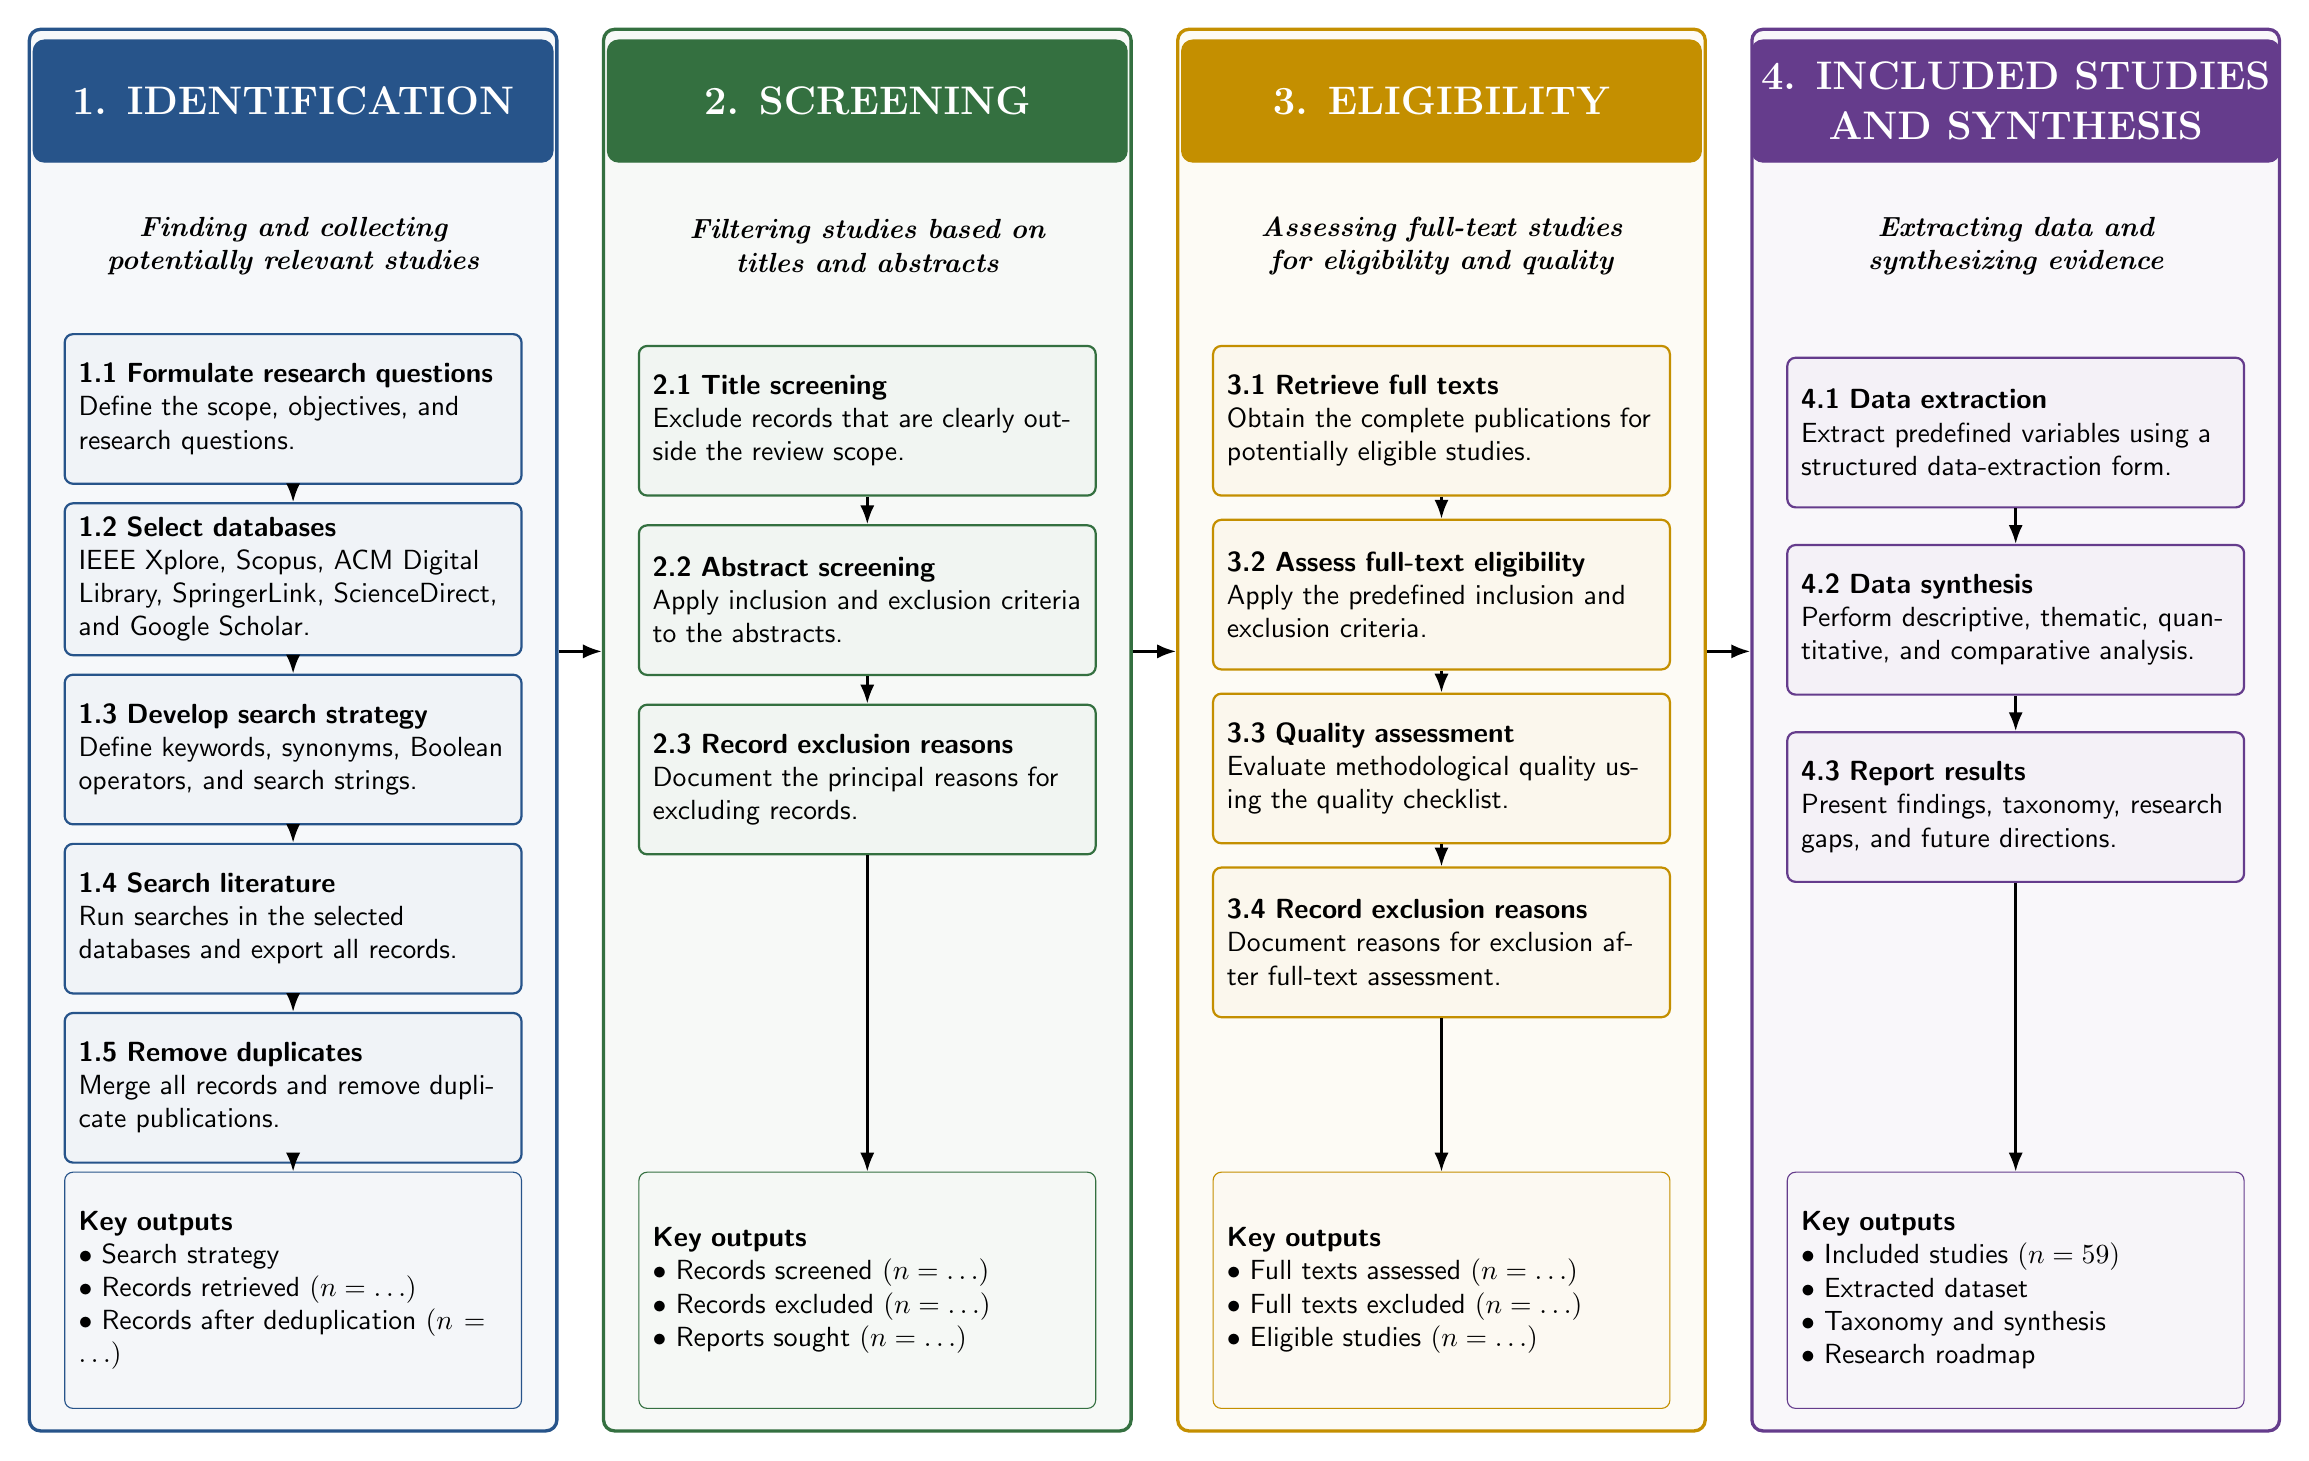
\begin{tikzpicture}[
    font=\sffamily,
    phase/.style={
        rounded corners=4pt,
        draw=#1,
        very thick,
        fill=#1!4,
        minimum width=6.7cm,
        minimum height=17.8cm
    },
    header/.style={
        rounded corners=4pt,
        draw=#1,
        fill=#1,
        text=white,
        font=\bfseries\Large,
        minimum width=6.6cm,
        minimum height=1.55cm,
        align=center
    },
    purpose/.style={
        font=\bfseries\itshape,
        text width=5.55cm,
        align=center,
        minimum height=1.5cm
    },
    step/.style={
        rounded corners=3pt,
        draw=#1,
        fill=#1!7,
        line width=0.8pt,
        text width=5.45cm,
        minimum height=1.9cm,
        inner sep=5pt,
        align=left
    },
    output/.style={
        rounded corners=3pt,
        draw=#1,
        fill=#1!5,
        text width=5.45cm,
        minimum height=3.0cm,
        inner sep=5pt,
        align=left
    },
    flow/.style={
        -{Latex[length=2.4mm]},
        line width=0.9pt
    }
]

\definecolor{identblue}{RGB}{39,84,138}
\definecolor{screengreen}{RGB}{52,112,64}
\definecolor{eliggold}{RGB}{196,143,0}
\definecolor{synthpurple}{RGB}{101,60,140}

% ============================================================
% PHASE PANELS
% ============================================================

\node[phase=identblue] (p1) at (0,0) {};
\node[phase=screengreen, right=0.55cm of p1] (p2) {};
\node[phase=eliggold, right=0.55cm of p2] (p3) {};
\node[phase=synthpurple, right=0.55cm of p3] (p4) {};

% ============================================================
% HEADERS
% ============================================================

\node[header=identblue, anchor=north]
    (h1) at ([yshift=-0.15cm]p1.north)
    {1. IDENTIFICATION};

\node[header=screengreen, anchor=north]
    (h2) at ([yshift=-0.15cm]p2.north)
    {2. SCREENING};

\node[header=eliggold, anchor=north]
    (h3) at ([yshift=-0.15cm]p3.north)
    {3. ELIGIBILITY};

\node[header=synthpurple, anchor=north]
    (h4) at ([yshift=-0.15cm]p4.north)
    {4. INCLUDED STUDIES\\AND SYNTHESIS};

% ============================================================
% PURPOSE STATEMENTS
% ============================================================

\node[purpose, below=0.30cm of h1]
    (pu1)
    {Finding and collecting\\potentially relevant studies};

\node[purpose, below=0.30cm of h2]
    (pu2)
    {Filtering studies based on\\titles and abstracts};

\node[purpose, below=0.30cm of h3]
    (pu3)
    {Assessing full-text studies\\for eligibility and quality};

\node[purpose, below=0.30cm of h4]
    (pu4)
    {Extracting data and\\synthesizing evidence};

% ============================================================
% IDENTIFICATION
% ============================================================

\node[step=identblue, below=0.35cm of pu1] (id1) {
\textbf{1.1 Formulate research questions}\\
Define the scope, objectives, and research questions.
};

\node[step=identblue, below=0.22cm of id1] (id2) {
\textbf{1.2 Select databases}\\
IEEE Xplore, Scopus, ACM Digital Library, SpringerLink,
ScienceDirect, and Google Scholar.
};

\node[step=identblue, below=0.22cm of id2] (id3) {
\textbf{1.3 Develop search strategy}\\
Define keywords, synonyms, Boolean operators, and search strings.
};

\node[step=identblue, below=0.22cm of id3] (id4) {
\textbf{1.4 Search literature}\\
Run searches in the selected databases and export all records.
};

\node[step=identblue, below=0.22cm of id4] (id5) {
\textbf{1.5 Remove duplicates}\\
Merge all records and remove duplicate publications.
};

\node[output=identblue, anchor=south]
    (out1) at ([yshift=0.30cm]p1.south) {
\textbf{Key outputs}\\
$\bullet$ Search strategy\\
$\bullet$ Records retrieved $(n=\ldots)$\\
$\bullet$ Records after deduplication $(n=\ldots)$
};

\draw[flow] (id1) -- (id2);
\draw[flow] (id2) -- (id3);
\draw[flow] (id3) -- (id4);
\draw[flow] (id4) -- (id5);
\draw[flow] (id5) -- (out1);

% ============================================================
% SCREENING
% ============================================================

\node[step=screengreen, below=0.50cm of pu2] (sc1) {
\textbf{2.1 Title screening}\\
Exclude records that are clearly outside the review scope.
};

\node[step=screengreen, below=0.35cm of sc1] (sc2) {
\textbf{2.2 Abstract screening}\\
Apply inclusion and exclusion criteria to the abstracts.
};

\node[step=screengreen, below=0.35cm of sc2] (sc3) {
\textbf{2.3 Record exclusion reasons}\\
Document the principal reasons for excluding records.
};

\node[output=screengreen, anchor=south]
    (out2) at ([yshift=0.30cm]p2.south) {
\textbf{Key outputs}\\
$\bullet$ Records screened $(n=\ldots)$\\
$\bullet$ Records excluded $(n=\ldots)$\\
$\bullet$ Reports sought $(n=\ldots)$
};

\draw[flow] (sc1) -- (sc2);
\draw[flow] (sc2) -- (sc3);
\draw[flow] (sc3) -- (out2);

% ============================================================
% ELIGIBILITY
% ============================================================

\node[step=eliggold, below=0.50cm of pu3] (el1) {
\textbf{3.1 Retrieve full texts}\\
Obtain the complete publications for potentially eligible studies.
};

\node[step=eliggold, below=0.28cm of el1] (el2) {
\textbf{3.2 Assess full-text eligibility}\\
Apply the predefined inclusion and exclusion criteria.
};

\node[step=eliggold, below=0.28cm of el2] (el3) {
\textbf{3.3 Quality assessment}\\
Evaluate methodological quality using the quality checklist.
};

\node[step=eliggold, below=0.28cm of el3] (el4) {
\textbf{3.4 Record exclusion reasons}\\
Document reasons for exclusion after full-text assessment.
};

\node[output=eliggold, anchor=south]
    (out3) at ([yshift=0.30cm]p3.south) {
\textbf{Key outputs}\\
$\bullet$ Full texts assessed $(n=\ldots)$\\
$\bullet$ Full texts excluded $(n=\ldots)$\\
$\bullet$ Eligible studies $(n=\ldots)$
};

\draw[flow] (el1) -- (el2);
\draw[flow] (el2) -- (el3);
\draw[flow] (el3) -- (el4);
\draw[flow] (el4) -- (out3);

% ============================================================
% INCLUDED STUDIES AND SYNTHESIS
% ============================================================

\node[step=synthpurple, below=0.65cm of pu4] (in1) {
\textbf{4.1 Data extraction}\\
Extract predefined variables using a structured data-extraction form.
};

\node[step=synthpurple, below=0.45cm of in1] (in2) {
\textbf{4.2 Data synthesis}\\
Perform descriptive, thematic, quantitative, and comparative analysis.
};

\node[step=synthpurple, below=0.45cm of in2] (in3) {
\textbf{4.3 Report results}\\
Present findings, taxonomy, research gaps, and future directions.
};

\node[output=synthpurple, anchor=south]
    (out4) at ([yshift=0.30cm]p4.south) {
\textbf{Key outputs}\\
$\bullet$ Included studies $(n=59)$\\
$\bullet$ Extracted dataset\\
$\bullet$ Taxonomy and synthesis\\
$\bullet$ Research roadmap
};

\draw[flow] (in1) -- (in2);
\draw[flow] (in2) -- (in3);
\draw[flow] (in3) -- (out4);

% ============================================================
% CONNECTIONS BETWEEN PHASES
% ============================================================

\draw[flow]
    ([yshift=1.0cm]p1.east)
    -- ([yshift=1.0cm]p2.west);

\draw[flow]
    ([yshift=1.0cm]p2.east)
    -- ([yshift=1.0cm]p3.west);

\draw[flow]
    ([yshift=1.0cm]p3.east)
    -- ([yshift=1.0cm]p4.west);

\end{tikzpicture}%
}
\caption{PRISMA-oriented systematic review workflow used in this study.
The first three phases describe study identification, screening, and
eligibility assessment, while the final phase covers extraction,
synthesis, and reporting of the included evidence.}
\label{fig:review_workflow}
\end{figure*}
\begin{enumerate}
    \item Formulation of the \glspl{rq};
    \item Selection of digital literature databases;
    \item Development of the search strategy;
    \item Systematic literature retrieval;
    \item Duplicate detection and removal;
    \item Study selection using predefined inclusion and exclusion criteria;
    \item \gls{qa} of the selected studies;
    \item Structured data extraction;
    \item Qualitative and comparative data synthesis.
\end{enumerate}

%%%%%%%%%%%%%%%%%%%%%%%%%%%%%%%%%%%%%%%%%%%%%%%%%%%%%%%%%%%%%%%%%%%%%%%%%%%%%%

\subsection{Review Protocol}

A review protocol was defined before commencing the literature search to ensure the transparency, consistency, and reproducibility of the entire review process. The protocol specifies the research objectives, search strategy, study selection criteria, quality assessment procedure, data extraction framework, and synthesis methodology adopted in this study. Although the protocol was not formally registered in an external repository, all methodological decisions were established before the study selection process began.

Table~\ref{tab:protocol} summarizes the review protocol adopted in this work.

\begin{table}[!t]
\caption{Summary of the Review Protocol}
\label{tab:protocol}
\centering
\begin{tabular}{p{3.1cm}p{4.4cm}}
\toprule
\textbf{Item} & \textbf{Description} \\
\midrule
Review Method & \gls{prisma} 2020 \gls{slr} \\
Research Domain & \gls{dectnr} \\
Publication Period & January 2020 -- July 2026 \\
Language & English \\
Primary Databases & IEEE Xplore, Scopus, ACM Digital Library, SpringerLink, ScienceDirect \\
Complementary Search & Google Scholar (Backward and Forward Snowballing) \\
Search Fields & Title, Abstract, and Author Keywords \\
Duplicate Management & Zotero Reference Manager \\
Study Selection & \gls{prisma} Screening Process \\
Quality Assessment & Five quality criteria (0--10) \\
Data Extraction & Structured extraction template \\
Data Analysis & Descriptive, comparative, and thematic synthesis \\
\bottomrule
\end{tabular}
\end{table}

%%%%%%%%%%%%%%%%%%%%%%%%%%%%%%%%%%%%%%%%%%%%%%%%%%%%%%%%%%%%%%%%%%%%%%%%%%%%%%

\subsection{Research Questions}

The primary objective of this \gls{slr} is to provide a comprehensive overview of the current state of \gls{dectnr} research, identify emerging research trends, evaluate existing implementation and validation approaches, and highlight future research opportunities. To achieve these objectives, the review addresses the following \glspl{rq}.

\begin{itemize}

\item[\textbf{RQ1}] How has research on \gls{dectnr} evolved in terms of publication trends, publication types, publishers, and application domains?

\item[\textbf{RQ2}] Which technical aspects of \gls{dectnr}, including the \gls{phy}, \gls{mac}, routing, resource allocation, positioning, security, and industrial applications, have been investigated?

\item[\textbf{RQ3}] Which evaluation methodologies, implementation platforms, software tools, and hardware platforms have been employed to validate \gls{dectnr} systems?

\item[\textbf{RQ4}] Which \glspl{kpi} have been used to evaluate \gls{dectnr}, and what performance characteristics have been reported?

\item[\textbf{RQ5}] What are the principal scientific contributions and technical limitations reported in the existing literature?

\item[\textbf{RQ6}] Which research gaps remain insufficiently addressed in the current body of \gls{dectnr} literature?

\item[\textbf{RQ7}] What future research directions are most promising for advancing \gls{dectnr} towards large-scale \gls{iiot} deployments?

\end{itemize}
\subsection{Eligibility Criteria}

The inclusion and exclusion criteria were defined before the screening
process. A study was included if it satisfied all of the following criteria:

\begin{itemize}
    \item it primarily investigated \gls{dectnr} or DECT NR+;
    \item it presented a technical, experimental, analytical, architectural,
    or application-oriented contribution;
    \item it was written in English;
    \item the full text was available;
    \item it was published between January 2020 and July 2026;
    \item it provided sufficient methodological or technical detail to support
    data extraction.
\end{itemize}

A study was excluded if it:

\begin{itemize}
    \item mentioned \gls{dectnr} only briefly or as background;
    \item primarily addressed another wireless technology;
    \item was a duplicate record;
    \item lacked sufficient technical content;
    \item was not available in English;
    \item was an editorial, presentation slide set, poster, or non-technical
    document.
\end{itemize}

Studies that were relevant to the broader context of industrial wireless
communications but did not primarily focus on \gls{dectnr} were classified
as contextual studies and were excluded from the quantitative synthesis.
\subsection{Quality Assessment}

Each included study was assessed using five quality criteria:

\begin{enumerate}
    \item clarity of the research objective;
    \item appropriateness of the methodology;
    \item strength of the validation;
    \item clarity of the discussion and limitations;
    \item reproducibility of the study.
\end{enumerate}

Each criterion was scored on a three-point scale:

\begin{itemize}
    \item 0: criterion not addressed;
    \item 1: criterion partially addressed;
    \item 2: criterion fully addressed.
\end{itemize}

The total quality score therefore ranged from 0 to 10. Studies scoring
8--10 were classified as high quality, studies scoring 5--7 as moderate
quality, and studies scoring below 5 as low quality.
\subsection{Data Extraction}

A structured data extraction form was used to collect information from each
included study. The extracted fields comprised:

\begin{itemize}
    \item bibliographic information;
    \item publication year and publication type;
    \item primary and secondary research contributions;
    \item technical topics;
    \item evaluation methodology;
    \item hardware and software platforms;
    \item network topology and deployment environment;
    \item frequency band and bandwidth;
    \item evaluated \glspl{kpi};
    \item application domain;
    \item key findings;
    \item scientific contribution;
    \item limitations;
    \item identified research gaps;
    \item proposed future work.
\end{itemize}

The extracted information was stored in a structured spreadsheet database.
Binary one-hot coding was used for multi-label attributes such as technical
topics, evaluation methods, application domains, and performance metrics.
\subsection{Study Classification and Coding}

Each study was assigned exactly one primary contribution category, while
multiple secondary technical topics were allowed. This distinction prevented
double counting in the analysis of primary research contributions while
preserving the multidisciplinary nature of the literature.

Multi-label technical topics included the \gls{phy}, \gls{mac},
routing and mesh networking, scheduling and resource allocation,
positioning, security, energy efficiency, coexistence, artificial
intelligence, standardization, industrial applications, \gls{urllc},
and \gls{mmtc}.

Evaluation methodologies were coded independently as simulation,
analytical or mathematical modeling, experimental or testbed validation,
and survey or overview. A paper could therefore belong to more than one
methodological category.
\subsection{Reliability and Consistency Checks}

To improve coding reliability, the extracted data were reviewed in multiple
stages. Evaluation methods, technical topics, performance metrics, hardware
platforms, and application domains were cross-checked across the master
database and the corresponding binary classification matrices.

Where inconsistencies were identified, the full paper, abstract, methodology,
results, and conclusion sections were re-examined. The final database was
then frozen and used as the single source for all quantitative analyses,
tables, figures, and percentages reported in this review.
\subsection{Data Synthesis and Analysis}

The included studies were analyzed using descriptive, comparative, and
thematic synthesis.

Descriptive analysis was used to examine publication trends, publication
types, research categories, evaluation methods, hardware platforms,
application domains, and performance metrics.

Comparative analysis was used to examine differences between simulation-based,
analytical, and experimental studies.

Thematic synthesis was used to group the reported scientific contributions,
limitations, research gaps, and future research directions into recurring
themes.

Because technical topics, evaluation methods, and performance metrics were
coded as multi-label attributes, the corresponding percentages may sum to
more than 100\%.
\subsection{Threats to Validity}

Several threats to validity should be acknowledged. First, relevant studies
may have been missed because of differences in database indexing or search
terminology. This risk was reduced by searching multiple databases and
performing backward and forward snowballing.

Second, the classification of research topics and contributions involves
researcher judgment. To reduce subjectivity, a predefined coding framework
was applied consistently, and ambiguous cases were re-examined using the
full text.

Third, the rapidly evolving nature of \gls{dectnr} means that recently
accepted or presented papers may not yet be indexed in major databases.
Therefore, the review reflects the state of the literature up to July 2026.

Finally, some studies did not provide complete information about hardware,
software, datasets, or reproducibility, which limited the depth of certain
comparisons.

%%%%%%%%%%%%%%%%%%%%%%%%%%%%%%%%%%%%%%%%%%%%%%%%%%%%%%%%%%%%%%%%%%%%%%%%%%%%%%%%
\section{Results of the Systematic Literature Review}
\label{sec:results}
%%%%%%%%%%%%%%%%%%%%%%%%%%%%%%%%%%%%%%%%%%%%%%%%%%%%%%%%%%%%%%%%%%%%%%%%%%%%%%%%

This section presents the results of the systematic literature review conducted according to the methodology described in Section~\ref{sec:methodology}. The objective of this section is to quantitatively characterize the collected literature rather than to discuss the technical contributions of individual publications. Accordingly, the analysis focuses on the outcome of the literature search, bibliometric characteristics of the selected studies, research trends, technical topic distribution, evaluation methodologies, validation approaches, reported performance metrics, and implementation platforms. Together, these analyses provide a comprehensive overview of the current \gls{dectnr} research landscape and establish the foundation for the technical synthesis presented in Section~\ref{sec:technical_synthesis}.

%%%%%%%%%%%%%%%%%%%%%%%%%%%%%%%%%%%%%%%%%%%%%%%%%%%%%%%%%%%%%%%%%%%%%%%%%%%%%%%%
\subsection{Literature Search Results}
\label{subsec:search_results}
%%%%%%%%%%%%%%%%%%%%%%%%%%%%%%%%%%%%%%%%%%%%%%%%%%%%%%%%%%%%%%%%%%%%%%%%%%%%%%%%

The systematic literature search was performed in July~2026 following the review protocol presented in Section~\ref{sec:methodology}. Five major scientific databases, namely IEEE Xplore, Scopus, ACM Digital Library, SpringerLink, and ScienceDirect, were systematically searched using the predefined Boolean search query. In addition, Google Scholar was employed as a complementary search engine to support backward and forward snowballing and to identify relevant publications that were not indexed in the primary scientific databases. The complete study selection process followed the \gls{prisma} 2020 framework and is illustrated in Figure~\ref{fig:prisma}.

The initial database search identified 86 potentially relevant publications, comprising 42 publications retrieved from IEEE Xplore and 44 publications indexed in Scopus. No additional publications satisfying the predefined search criteria were identified in ACM Digital Library, SpringerLink, or ScienceDirect. Google Scholar returned a substantially larger number of search results; however, these were not considered part of the primary search dataset and were instead used exclusively for citation tracking and snowballing.

After removing duplicate records using Zotero Reference Manager, the remaining publications were screened according to the predefined inclusion and exclusion criteria. The screening process consisted of title screening, abstract screening, and full-text assessment. Publications unrelated to \gls{dectnr}, papers lacking sufficient technical content, inaccessible documents, and studies outside the scope of this review were excluded. Additional relevant publications identified through backward and forward snowballing were incorporated into the final literature corpus whenever they satisfied all eligibility criteria and were not already included in the primary database search.

The final dataset comprises 51 high-quality publications together with the relevant \gls{etsi} Technical Specifications, \gls{etsi} Technical Reports, and \gls{itur} recommendations that define the \gls{dectnr} standardization framework. Collectively, these documents capture the evolution of \gls{dectnr} from its initial standardization activities through protocol design, algorithm development, hardware implementation, experimental validation, and industrial deployment. This curated dataset forms the basis for the quantitative analyses presented in the following subsections and for the comprehensive technical synthesis provided in Section~\ref{sec:technical_synthesis}.

%%%%%%%%%%%%%%%%%%%%%%%%%%%%%%%%%%%%%%%%%%%%%%%%%%%%%%%%%%%%%%%%%%%%%%%%%%%%%%%%
\subsection{Bibliometric Analysis}
\label{subsec:bibliometric}
%%%%%%%%%%%%%%%%%%%%%%%%%%%%%%%%%%%%%%%%%%%%%%%%%%%%%%%%%%%%%%%%%%%%%%%%%%%%%%%%

To obtain a comprehensive understanding of the evolution of \gls{dectnr} research, the final literature corpus was analyzed from multiple bibliometric perspectives. Unlike the subsequent technical synthesis, which examines the technical contributions of the literature, the objective of this section is to characterize the research landscape quantitatively. The analysis investigates publication trends over time, publication types, primary research contributions, technical topic distribution, evaluation methodologies, validation approaches, reported performance metrics, and implementation platforms. These statistics provide valuable insights into the maturity of the research field, the dominant research directions, and the methodological evolution of the published literature.

%%%%%%%%%%%%%%%%%%%%%%%%%%%%%%%%%%%%%%%%%%%%%%%%%%%%%%%%%%%%%%%%%%%%%%%%%%%%%%%%
\subsubsection{Publication Trends}
\label{subsubsec:publication_trends}
%%%%%%%%%%%%%%%%%%%%%%%%%%%%%%%%%%%%%%%%%%%%%%%%%%%%%%%%%%%%%%%%%%%%%%%%%%%%%%%%

Figure~\ref{fig:publication_year} illustrates the annual distribution of the publications included in this systematic literature review. The figure clearly demonstrates the rapid growth of \gls{dectnr} research since the introduction of the technology. Following the publication of the earliest standardization activities in 2020, the number of scientific publications increased steadily during the subsequent years, reflecting the growing academic and industrial interest in the technology.

The publication trend indicates three distinct phases in the evolution of the research field. The first phase (2020--2022) was characterized primarily by standardization activities, architectural design, and the establishment of the fundamental communication framework. During this period, research focused on defining the protocol architecture, physical layer, medium access control procedures, and demonstrating compliance with the \gls{imt2020} requirements. The second phase (2023) represents a transition toward implementation-oriented research, during which the availability of development platforms enabled the first experimental investigations and practical demonstrations. The third phase (2024--2026) exhibits a substantial increase in research activity, with publications expanding toward protocol optimization, localization, routing, scheduling, industrial applications, hardware implementations, and large-scale experimental evaluations.

The apparent reduction in the number of publications during 2026 should not be interpreted as a decline in research activity. Instead, it reflects the fact that the literature search was conducted during the middle of the publication year, and therefore many conference proceedings and journal articles scheduled for publication later in the year were not yet available. Overall, the observed publication trend demonstrates that \gls{dectnr} has rapidly evolved from a newly standardized radio interface into an active and expanding research field attracting increasing attention from both academia and industry.

%%%%%%%%%%%%%%%%%%%%%%%%%%%%%%%%%%%%%%%%%%%%%%%%%%%%%%%%%%%%%%%%%%%%%%%%%%%%%%%%
\subsubsection{Publication Types}
\label{subsubsec:publication_types}
%%%%%%%%%%%%%%%%%%%%%%%%%%%%%%%%%%%%%%%%%%%%%%%%%%%%%%%%%%%%%%%%%%%%%%%%%%%%%%%%

The distribution of publication types is presented in Figure~\ref{fig:publication_types}. Conference papers constitute the dominant publication venue, accounting for the majority of the included studies, whereas journal articles, survey papers, and academic theses represent comparatively smaller proportions of the literature.

This distribution reflects the relatively recent emergence of \gls{dectnr} as an \gls{imt2020} radio interface. Newly developing wireless communication technologies are typically disseminated first through international conferences, where researchers rapidly communicate novel algorithms, protocol enhancements, hardware implementations, and experimental results. Journal publications generally appear later as the technology matures and more comprehensive validation studies become available. Consequently, the predominance of conference publications observed in this review is consistent with the current developmental stage of the technology.

The presence of several survey papers further indicates that the research community has begun consolidating knowledge across individual technical domains. Nevertheless, the relatively limited number of comprehensive surveys demonstrates that the research landscape is still evolving, thereby motivating the need for a systematic literature review that integrates standardization documents, protocol developments, implementation studies, and experimental evaluations into a unified analytical framework.
%%%%%%%%%%%%%%%%%%%%%%%%%%%%%%%%%%%%%%%%%%%%%%%%%%%%%%%%%%%%%%%%%%%%%%%%%%%%%%%%
\subsection{Research Characteristics}
\label{subsec:research_characteristics}
%%%%%%%%%%%%%%%%%%%%%%%%%%%%%%%%%%%%%%%%%%%%%%%%%%%%%%%%%%%%%%%%%%%%%%%%%%%%%%%%

Beyond the bibliometric evolution of the literature, the selected publications were further analyzed according to their primary research contributions, technical focus areas, evaluation methodologies, validation approaches, reported performance metrics, and implementation platforms. Unlike conventional bibliometric indicators, these characteristics provide insight into how the \gls{dectnr} research community has progressed from standardization activities toward algorithm development, implementation, experimental validation, and industrial deployment. Collectively, these analyses reveal the maturity of the research field and identify the dominant methodological trends that have shaped the evolution of \gls{dectnr}.

%%%%%%%%%%%%%%%%%%%%%%%%%%%%%%%%%%%%%%%%%%%%%%%%%%%%%%%%%%%%%%%%%%%%%%%%%%%%%%%%
\subsubsection{Primary Research Contributions}
\label{subsubsec:primary_contributions}
%%%%%%%%%%%%%%%%%%%%%%%%%%%%%%%%%%%%%%%%%%%%%%%%%%%%%%%%%%%%%%%%%%%%%%%%%%%%%%%%

Figure~\ref{fig3} classifies each publication according to its primary scientific contribution. The results indicate that the current research landscape is dominated by industrial applications, physical-layer techniques, and medium access control mechanisms, which together represent the largest proportion of the available literature. These research areas constitute the technological foundation of \gls{dectnr} and therefore received considerable attention during the early stages of the technology's development.

A substantial number of publications also focus on standardization activities, routing and mesh networking, and analytical modeling, reflecting the continued evolution of the protocol stack beyond the initial \gls{etsi} specifications. In contrast, comparatively fewer studies investigate scheduling and resource allocation, localization, security, and multi-radio interoperability. Although these research topics have attracted increasing interest in recent years, they remain comparatively underexplored relative to the core communication protocols. This distribution suggests that future research is expected to expand toward higher-layer optimization, intelligent resource management, and cross-layer communication techniques as the technology continues to mature.

%%%%%%%%%%%%%%%%%%%%%%%%%%%%%%%%%%%%%%%%%%%%%%%%%%%%%%%%%%%%%%%%%%%%%%%%%%%%%%%%
\subsubsection{Technical Topic Coverage}
\label{subsubsec:technical_topics}
%%%%%%%%%%%%%%%%%%%%%%%%%%%%%%%%%%%%%%%%%%%%%%%%%%%%%%%%%%%%%%%%%%%%%%%%%%%%%%%%

The multi-label classification presented in Figure~\ref{fig4} provides a broader perspective on the technical coverage of the reviewed literature. Unlike the primary contribution analysis, individual publications may contribute to multiple technical domains simultaneously, thereby illustrating the interdisciplinary nature of \gls{dectnr} research.

The analysis demonstrates that physical-layer techniques, medium access control, routing and mesh networking, and experimental applications constitute the most extensively investigated research areas. Considerable research activity is also observed in standardization, \gls{urllc}, energy-efficient communication, and positioning technologies, highlighting the growing diversification of the research landscape. Conversely, comparatively limited attention has been devoted to queue management, artificial intelligence-assisted networking, backscatter communication, and advanced resource allocation mechanisms. These findings indicate that while the fundamental communication architecture has reached a relatively mature stage, several higher-layer optimization topics remain open research directions.

%%%%%%%%%%%%%%%%%%%%%%%%%%%%%%%%%%%%%%%%%%%%%%%%%%%%%%%%%%%%%%%%%%%%%%%%%%%%%%%%
\subsubsection{Evaluation Methodologies}
\label{subsubsec:evaluation_methods}
%%%%%%%%%%%%%%%%%%%%%%%%%%%%%%%%%%%%%%%%%%%%%%%%%%%%%%%%%%%%%%%%%%%%%%%%%%%%%%%%

Figure~\ref{fig5} summarizes the evaluation methodologies adopted by the reviewed publications. Simulation represents the dominant evaluation approach, followed by analytical modeling and experimental validation. Survey papers constitute a comparatively smaller proportion of the literature, reflecting the relatively recent emergence of \gls{dectnr} research.

The predominance of simulation-based studies is consistent with the early development phase of a new wireless communication technology, where protocol verification, algorithm evaluation, and system optimization are typically performed before large-scale hardware implementation becomes widely available. Nevertheless, the significant number of experimental studies demonstrates that the research community has increasingly shifted toward practical validation using prototype hardware, software-defined radio platforms, commercial devices, and industrial testbeds. This transition illustrates the progressive maturation of \gls{dectnr} from theoretical protocol design toward practical deployment.

%%%%%%%%%%%%%%%%%%%%%%%%%%%%%%%%%%%%%%%%%%%%%%%%%%%%%%%%%%%%%%%%%%%%%%%%%%%%%%%%
\subsubsection{Validation Approaches}
\label{subsubsec:validation_approaches}
%%%%%%%%%%%%%%%%%%%%%%%%%%%%%%%%%%%%%%%%%%%%%%%%%%%%%%%%%%%%%%%%%%%%%%%%%%%%%%%%

To further characterize the maturity of the published research, the experimental studies were classified according to their validation approaches, as illustrated in Figure~\ref{fig6}. Hardware prototypes constitute the most frequently employed validation platform, followed by commercial devices, numerical simulations, and system-level simulations. Link-level simulations, field trials, software-defined radio implementations, and industrial measurements are also represented within the reviewed literature.

The diversity of validation methodologies demonstrates that \gls{dectnr} research has progressed beyond purely theoretical investigations. The increasing availability of commercial chipsets, embedded development platforms, and industrial prototype systems has enabled researchers to evaluate protocol implementations under realistic operating conditions. Although large-scale industrial deployments remain comparatively limited, the growing number of hardware-based validation studies indicates that the technology has entered an important phase of practical implementation and experimental verification.

%%%%%%%%%%%%%%%%%%%%%%%%%%%%%%%%%%%%%%%%%%%%%%%%%%%%%%%%%%%%%%%%%%%%%%%%%%%%%%%%
\subsubsection{Reported Performance Metrics}
\label{subsubsec:performance_metrics}
%%%%%%%%%%%%%%%%%%%%%%%%%%%%%%%%%%%%%%%%%%%%%%%%%%%%%%%%%%%%%%%%%%%%%%%%%%%%%%%%

Figure~\ref{fig7} summarizes the performance metrics reported throughout the reviewed literature. Packet error rate, energy consumption, latency, reliability, and bit error rate are the most frequently evaluated performance indicators, emphasizing the importance of communication reliability and robustness in the design objectives of \gls{dectnr}. Additional metrics including throughput, communication coverage, received signal strength, signal-to-noise ratio, fairness, localization accuracy, and connection density are reported less frequently, while resource utilization and spectral efficiency receive comparatively limited attention.

The observed distribution reflects the current priorities of the research community. Existing studies primarily focus on demonstrating reliable communication, validating protocol correctness, and satisfying the stringent performance requirements associated with industrial wireless communication systems. In contrast, comparatively fewer publications investigate higher-level network optimization metrics such as fairness, resource utilization, and intelligent scheduling. These observations suggest that future research will increasingly address communication efficiency and resource optimization as the technology matures and larger-scale deployments become available.

%%%%%%%%%%%%%%%%%%%%%%%%%%%%%%%%%%%%%%%%%%%%%%%%%%%%%%%%%%%%%%%%%%%%%%%%%%%%%%%%
\subsubsection{Implementation Platforms}
\label{subsubsec:implementation_platforms}
%%%%%%%%%%%%%%%%%%%%%%%%%%%%%%%%%%%%%%%%%%%%%%%%%%%%%%%%%%%%%%%%%%%%%%%%%%%%%%%%

The implementation platforms employed in the reviewed studies are summarized in Figure~\ref{fig8}. Nordic Semiconductor's nRF91 platform represents the most widely adopted hardware platform for experimental \gls{dectnr} implementations, reflecting its availability as one of the first commercial development platforms supporting the technology. MATLAB remains the dominant software environment for analytical modeling and simulation-based evaluations, while FPGA implementations, GNU Radio, USRP-based software-defined radio platforms, Zephyr, and open-source software frameworks are employed in a smaller number of studies.

The diversity of implementation platforms demonstrates the continued evolution of \gls{dectnr} from algorithmic research toward practical system development. Software simulation environments remain essential for protocol analysis and performance evaluation, whereas commercial embedded platforms increasingly enable real-world experimentation and industrial validation. This combination of software- and hardware-based research provides strong evidence that the technology is transitioning from standardization and theoretical development toward practical deployment in industrial communication systems.
\begin{figure}[!t]
    \centering
    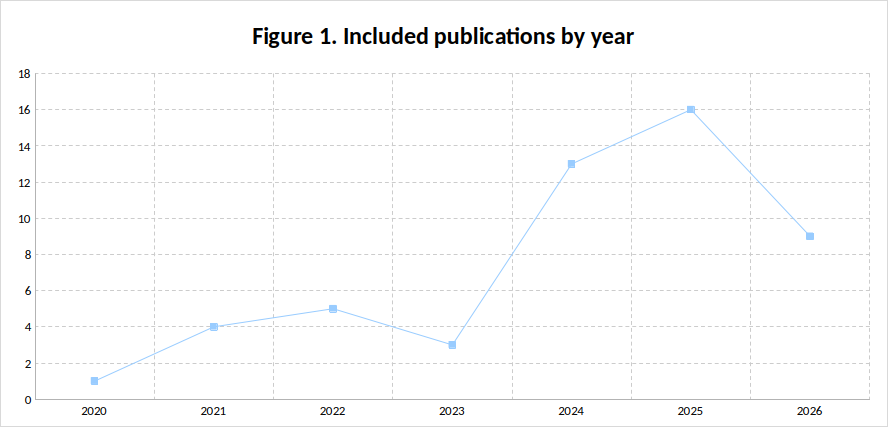
\includegraphics[width=\columnwidth]{figures/fig1.png}
    \caption{Annual distribution of the included DECT-2020 NR publications.}
    \label{fig1}
\end{figure}
\begin{figure}[!t]
    \centering
    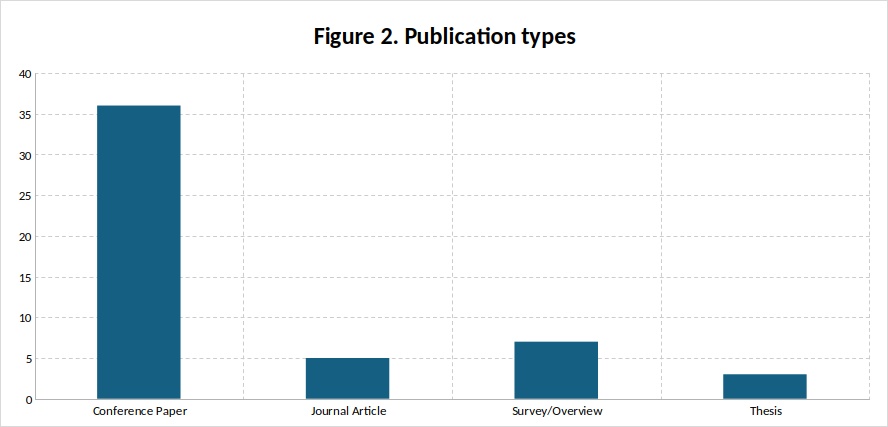
\includegraphics[width=\columnwidth]{figures/fig2.png}
    \caption{Annual distribution of the included DECT-2020 NR publications.}
    \label{fig2}
\end{figure}
\begin{figure}[!t]
    \centering
    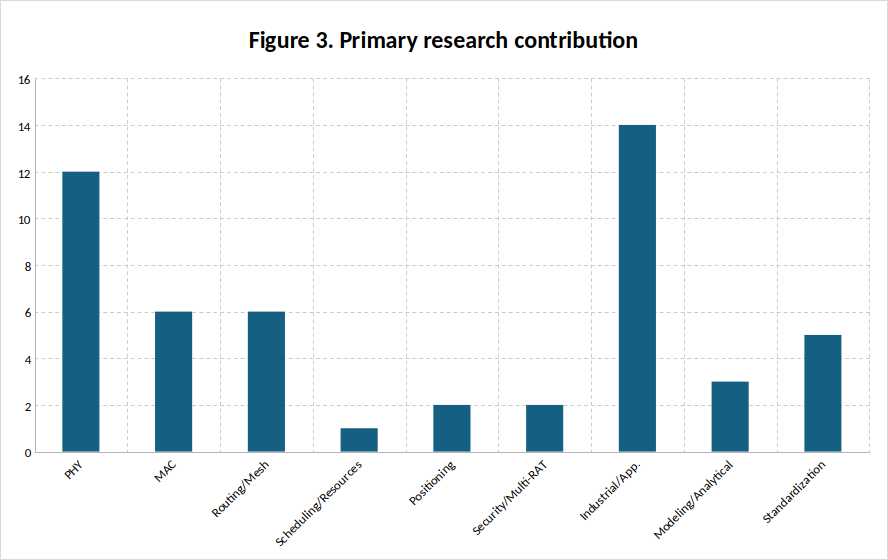
\includegraphics[width=\columnwidth]{figures/fig3.png}
    \caption{Annual distribution of the included DECT-2020 NR publications.}
    \label{fig3}
\end{figure}
\begin{figure}[!t]
    \centering
    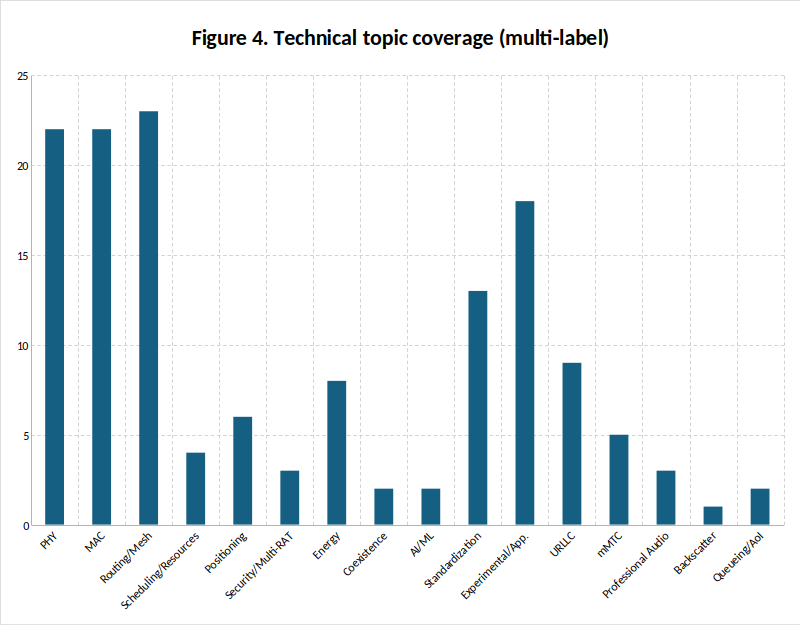
\includegraphics[width=\columnwidth]{figures/fig4.png}
    \caption{Annual distribution of the included DECT-2020 NR publications.}
    \label{fig4}
\end{figure}
\begin{figure}[!t]
    \centering
    
\includegraphics[width=\columnwidth]{figures/fig5.png}
    \caption{Annual distribution of the included DECT-2020 NR publications.}
    \label{fig5}
\end{figure}
\begin{figure}[!t]
    \centering
    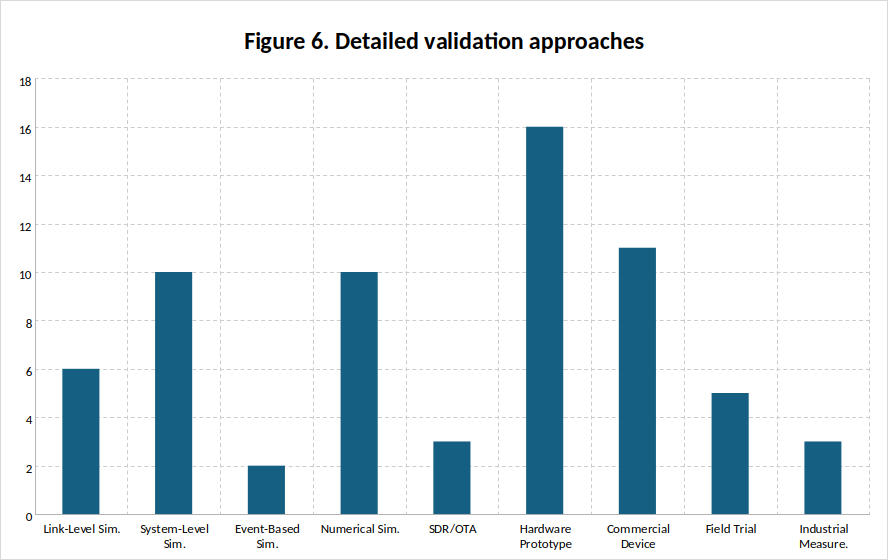
\includegraphics[width=\columnwidth]{figures/fig6.png}
    \caption{Annual distribution of the included DECT-2020 NR publications.}
    \label{fig6}
\end{figure}
\begin{figure}[!t]
    \centering
    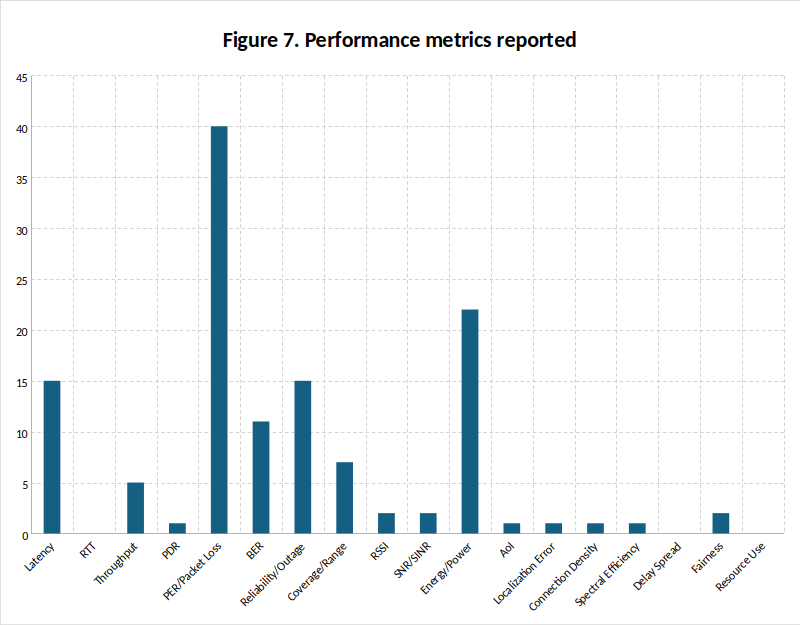
\includegraphics[width=\columnwidth]{figures/fig7.png}
    \caption{Annual distribution of the included DECT-2020 NR publications.}
    \label{fig7}
\end{figure}
\begin{figure}[!t]
    \centering
    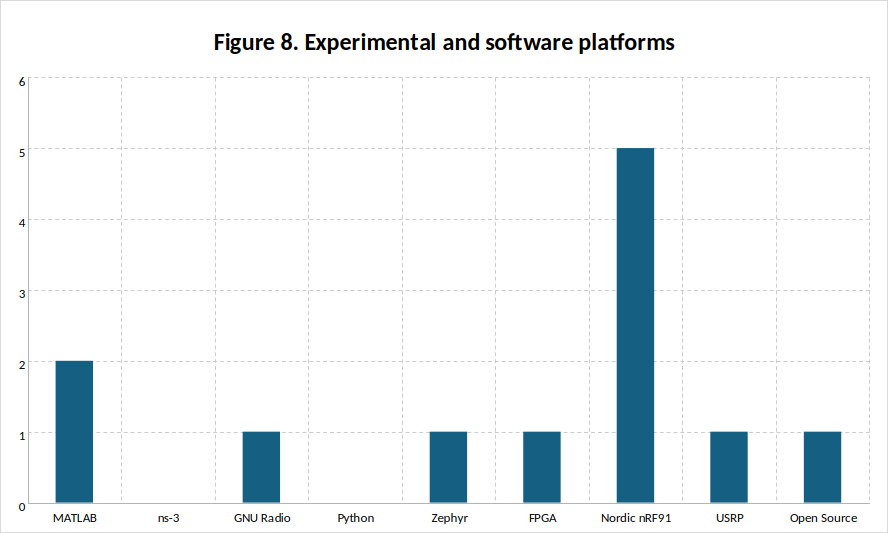
\includegraphics[width=\columnwidth]{figures/fig8.png}
    \caption{Annual distribution of the included DECT-2020 NR publications.}
    \label{fig8}
\end{figure}
%%%%%%%%%%%%%%%%%%%%%%%%%%%%%%%%%%%%%%%%%%%%%%%%%%%%%%%%%%%%%%%%%%%%%%%%%%%%%%%%
\section{Technical Synthesis of DECT-2020 NR Research}
\label{sec:technical_synthesis}

The quantitative results presented in Section~\ref{sec:results} describe the
distribution of the reviewed literature across publication characteristics,
technical topics, methodologies, and evaluation approaches. This section
complements that quantitative analysis with a technical synthesis of the
51 included primary studies. Based on their principal technical contributions,
the literature is organized into the research taxonomy shown in
Figure~\ref{fig:research_taxonomy}. The taxonomy provides the structure for the
subsequent analysis while recognizing that individual studies may contribute
to multiple research areas.

\begin{figure*}[t]
    \centering
    
\includegraphics[width=\textwidth]{figures/ResearchTexanomy.png}
    \caption{Taxonomy of the DECT-2020 NR research landscape derived from the
    qualitative synthesis of the 51 included primary studies. The taxonomy
    organizes the literature into ten principal research areas while allowing
    individual studies to address multiple areas.}
    \label{fig:research_taxonomy}
\end{figure*}

%%%%%%%%%%%%%%%%%%%%%%%%%%%%%%%%%%%%%%%%%%%%%%%%%%%%%%%%%%%%%%%%%%%%%%%%%%%%%%%%
%%%%%%%%%%%%%%%%%%%%%%%%%%%%%%%%%%%%%%%%%%%%%%%%%%%%%%%%%%%%%%%%%%%%%%%%%%%%%%%%
%%%%%%%%%%%%%%%%%%%%%%%%%%%%%%%%%%%%%%%%%%%%%%%%%%%%%%%%%%%%%%%%%%%%%%%%%%%%%%%%
\subsection{Standardization and System Architecture}
\label{subsec:standardization_architecture}
%%%%%%%%%%%%%%%%%%%%%%%%%%%%%%%%%%%%%%%%%%%%%%%%%%%%%%%%%%%%%%%%%%%%%%%%%%%%%%%%

The standardization and architectural foundations of \gls{dectnr} provide the
basis for subsequent research on the \gls{phy}, \gls{mac}, routing, resource
management, and industrial applications. As shown in
Section~\ref{subsec:technical_landscape}, five studies in the final corpus were
classified primarily as standardization or overview contributions, while
architectural aspects recur across several other technical categories
\cite{kovalchukovDECT2020NewRadio2022,
perez-guiraoDECTNRUnveiling2022,
maliatsosEvaluationIMT2020Candidate2022a,
smidaETSIDECT2020Component2023}.

The development of \gls{dectnr} was closely associated with the
\gls{imt2020} standardization process. The \gls{itur} established the
IMT-2020 vision, minimum performance requirements, and evaluation methodology
through ITU-R M.2083, M.2410, and M.2412
\cite{itur_m2083,itur_m2410,itur_m2412}. DECT-2020 NR was subsequently
evaluated as a candidate \gls{rit}, particularly for \gls{urllc} and
\gls{mmtc}, and its inclusion in Recommendation ITU-R M.2150 established it
as an IMT-2020 radio interface
\cite{itur_m2150,maliatsosEvaluationIMT2020Candidate2022a,
smidaETSIDECT2020Component2023}. Early studies therefore focused on
specification-level evaluation and compliance with the IMT-2020 framework,
providing the baseline for later protocol- and application-oriented research
\cite{maliatsosEvaluationIMT2020Candidate2022a,
smidaETSIDECT2020Component2023}.

The \gls{dectnr} specification is organized as a modular protocol family.
ETSI TS~103~636-1 defines the general system description and terminology,
Part~2 the radio requirements, Part~3 the \gls{phy}, Part~4 the \gls{mac},
and Part~5 the data-link-control and convergence functionality
\cite{etsi_ts103636_1,etsi_ts103636_2,etsi_ts103636_3,
etsi_ts103636_4,etsi_ts103636_5}. Complementary technical reports document
IMT-2020 evaluation and additional technical and regulatory aspects
\cite{etsi_tr103810,etsi_tr103943}. Together, these specifications provide
the protocol framework underlying the technical research synthesized in the
following subsections.

Beyond introducing a new radio interface, DECT NR+ adopts a decentralized and
flexible architecture designed for dense machine-type and vertical
communication
\cite{kovalchukovDECT2020NewRadio2022,
perez-guiraoDECTNRUnveiling2022}. Montalvo et al. place this development within
the broader evolution of the DECT family, from classical cordless
communication and DECT-ULE toward the multicarrier, OFDM-based DECT-2020 NR
interface developed for substantially different connectivity and performance
requirements
\cite{montalvoDECTEvolutionMeeting2024}.

A fundamental architectural element is the distinction between the logical
Fixed Termination (FT) and Portable Termination (PT) roles. An FT provides
control and radio-resource information, whereas PTs discover and associate
with an FT and use the available communication resources. These are logical
protocol roles rather than permanently assigned hardware classes, allowing
devices to support different roles according to their network function
\cite{etsi_ts103636_1,etsi_ts103636_4,
kovalchukovDECT2020NewRadio2022,
perez-guiraoDECTNRUnveiling2022}. This flexibility enables point-to-point and
local cluster communication as well as hierarchical and mesh-oriented
multi-hop structures in which combined FT/PT devices extend connectivity
without requiring every device to maintain a direct link to centralized
infrastructure
\cite{etsi_ts103636_1,etsi_ts103636_4,
kovalchukovDECT2020NewRadio2022,
perez-guiraoDECTNRUnveiling2022}.

\begin{figure*}[!t]
    \centering
    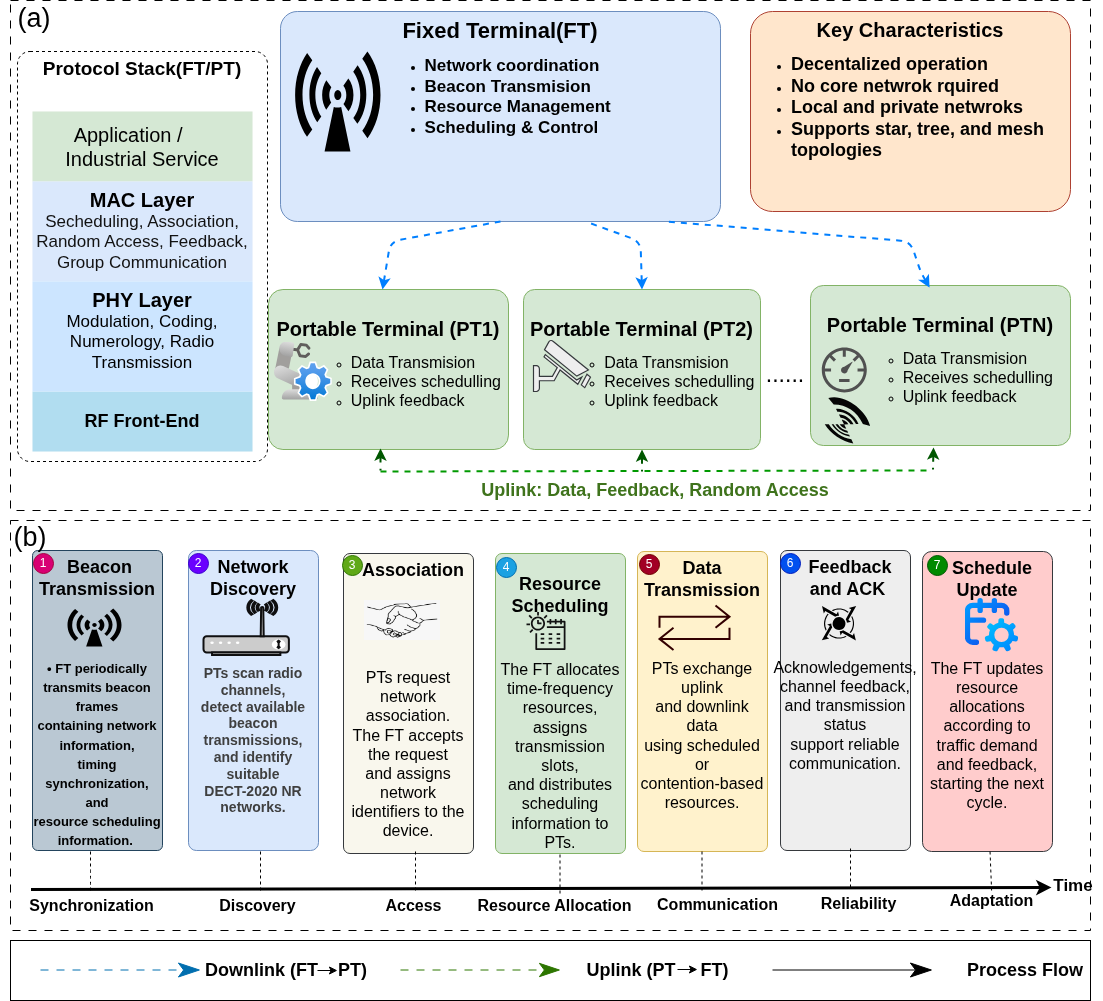
\includegraphics[width=0.95\textwidth]{figures/archetictur.png}
    \caption{Conceptual \gls{dectnr} architecture and representative
    communication workflow, illustrating logical FT/PT roles, network
    formation, resource coordination, association, data transmission, and
    feedback procedures.}
    \label{fig:dectnr_architecture}
\end{figure*}

Network formation is supported through standardized discovery, beaconing,
association, random-access, and resource-allocation procedures. FTs advertise
the information required for network discovery and radio operation, while PTs
use this information to associate and access communication resources. The
\gls{phy} and \gls{mac} additionally define channel observation, resource
selection, feedback, retransmission, and radio-resource coordination
\cite{etsi_ts103636_3,etsi_ts103636_4}. These mechanisms form the basis for
the channel-access and scheduling strategies examined later in the literature.

The flexibility of the FT/PT model is particularly important for multi-hop
operation. Ahmad et al. exploit dynamic roles and intermediate relays to
reconnect devices in outage regions, reporting an outage probability below
1\% under the evaluated simulation conditions
\cite{ahmadMACProtocolReducing2024}. Subsequent routing research investigates
selective forwarding, source routing, and topology-aware route selection,
illustrating how the standardized architecture can support different
multi-hop strategies
\cite{fuhrlingRobustRoutingProtocol2025b}.

Spectrum access is another important architectural characteristic.
\gls{dectnr} supports locally deployed networks through channel observation,
selection, and interference-management procedures
\cite{etsi_ts103636_2,etsi_ts103636_3,etsi_ts103636_4}.
Coexistence studies show that these mechanisms can support spectrum sharing
with existing DECT systems under the evaluated traffic and interference
conditions
\cite{samuylovPerformanceAssessmentDECT20202023}. Local spectrum operation
therefore increases deployment flexibility while making distributed
interference and resource management important aspects of practical network
operation.

The architecture also separates local radio connectivity from external-network
connectivity. Standardized convergence functionality enables local
device-to-device and multi-hop communication to be connected through selected
devices or gateways to higher-layer and external networks
\cite{etsi_ts103636_5}. Recent multi-RAT research exploits this property by
integrating \gls{dectnr} with other radio technologies and external
infrastructure
\cite{dangUniRATUnifiedDECT20202026}.

Overall, three architectural characteristics shape much of the subsequent
research: flexible FT/PT roles, decentralized local network formation, and
direct and multi-hop communication
\cite{kovalchukovDECT2020NewRadio2022,
perez-guiraoDECTNRUnveiling2022,
ahmadMACProtocolReducing2024,
fuhrlingRobustRoutingProtocol2025b}. These characteristics distribute
resource selection, association, forwarding, interference management, and
topology maintenance across participating devices, thereby coupling the
research problems addressed at different protocol layers. Consequently,
studies of channel access, routing, reliability, energy, and resource
management build on a common architectural foundation
\cite{samuylovPerformanceMACLayer2024a,
fuhrlingRobustRoutingProtocol2025b,
samuylovEmpoweringNearURLLCIoT2025,
bandaraExperimentalValidationAnalysis2025,
grafParetoOptimalityApproach2026a}.

%%%%%%%%%%%%%%%%%%%%%%%%%%%%%%%%%%%%%%%%%%%%%%%%%%%%%%%%%%%%%%%%%%%%%%%%%%%%%%%%
%%%%%%%%%%%%%%%%%%%%%%%%%%%%%%%%%%%%%%%%%%%%%%%%%%%%%%%%%%%%%%%%%%%%%%%%%%%%%%%%
\subsection{Physical-Layer Research}
\label{subsec:phy}
%%%%%%%%%%%%%%%%%%%%%%%%%%%%%%%%%%%%%%%%%%%%%%%%%%%%%%%%%%%%%%%%%%%%%%%%%%%%%%%%

Physical-layer research constitutes one of the most extensively investigated
areas of \gls{dectnr}. As shown in Section~\ref{sec:results}, 12 studies were
classified primarily as \gls{phy} contributions, while 22 of the 51 included
studies addressed PHY-related aspects. The literature progresses from
standard-oriented link-level evaluation toward comparative analysis,
propagation and industrial measurements, receiver implementation,
commercial-hardware experimentation, and adaptive transmission-parameter
selection.

The \gls{dectnr} \gls{phy} uses cyclic-prefix orthogonal
frequency-division multiplexing and supports configurable subcarrier spacing,
bandwidth, packet duration, modulation and coding, and transmission power.
These parameters jointly determine trade-offs among data rate, latency,
reliability, propagation robustness, and energy consumption
\cite{etsi_ts103636_2,etsi_ts103636_3,
perez-guiraoDECTNRUnveiling2022,
grafWhatExpectWhen2026,
grafParetoOptimalityApproach2026a}. In particular, higher MCS levels increase
payload capacity under favorable channel conditions, whereas more robust
configurations improve link reliability at the expense of transmission
efficiency.

Early PHY investigations were closely associated with IMT-2020 evaluation.
Penner et al. established link-level performance under standardized ITU-R
channel models for \gls{urllc} and \gls{mmtc}
\cite{pennerLinkLevelPerformanceEvaluation2021}. Subsequent studies evaluated
latency, reliability, connection density, and broader compliance with the
candidate-radio-interface requirements
\cite{dhanwaniAssessmentCandidateTechnology2020,
pennerURLLCPerformanceEvaluation2021,
maliatsosEvaluationIMT2020Candidate2022a,
smidaETSIDECT2020Component2023}. These studies provided the initial
simulation-based evidence for the radio interface before commercial DECT NR+
hardware became widely available.

Comparative and extended PHY studies subsequently explored the operating
characteristics of DECT NR+. Kizilirmak and Askarov compare DECT-2020 NR with
LTE-M and show the contrasting coverage--throughput objectives of the two
technologies. Under their modeled assumptions, coded BPSK at a BER of
$10^{-3}$ provides approximately 2.4~km for DECT-2020 NR compared with
approximately 7--8~km for LTE-M, although these values are model-dependent
rather than deployment guarantees
\cite{kizilirmakExaminationPHYLayer2024}. Leugner and Hellbrueck extend this
comparative perspective toward low-power wide-area networking by evaluating
DECT NR+ as an alternative to sub-GHz LPWAN technologies. Their study combines
modeled and experimental evaluation and highlights the trade-off between
communication range, data rate, and the use of higher-frequency spectrum
\cite{leugnerAlternativeSubGHzLPWAN2025a}. Soni et al. investigate
power-domain NOMA for multi-hop DECT-2020 NR and evaluate BER, outage
probability, and spectral efficiency, illustrating the potential of
alternative multiple-access techniques in dense multi-hop scenarios
\cite{soniLinkLevelAssessmentNOMA2023}.

Propagation and industrial-environment studies demonstrate the difference
between standardized link-level performance and practical radio behavior.
Haque et al. report packet success rates above 90\% for indoor non-line-of-sight
links beyond 60~m at 0~dBm and outdoor line-of-sight links beyond 600~m at
19~dBm
\cite{haqueDECT2020NRLink2025}. Llaguno et al. show through
factory-oriented simulations that PHY performance alone is insufficient to
guarantee stringent industrial reliability and must be complemented by
higher-layer control mechanisms
\cite{llagunoPhysicalLayerPerformance2024}. Wa{\ss}mann et al. further
evaluate DECT-2020 NR at 450, 1350, and 3700~MHz using bandwidths from
1.728 to 13.824~MHz in an industrial environment and report an average RMS
delay spread of approximately 65~ns for the 13.824~MHz configuration
\cite{wassmannPerformanceDECT2020NR2024}. Their results also reveal
hardware-dependent differences between frequency bands. Collectively, these
studies show that path loss, multipath, antenna placement, operating
frequency, radio hardware, transmission power, and MCS jointly determine
practical link performance
\cite{haqueDECT2020NRLink2025,
llagunoPhysicalLayerPerformance2024,
wassmannPerformanceDECT2020NR2024}.
Channel estimation represents a complementary PHY research direction,
particularly for challenging industrial propagation conditions. Liu et al.
investigate data-aided channel estimation for robust DECT NR+ links in
oil-and-gas equipment communication and combine simulation with laboratory
validation. Their results demonstrate how data-assisted channel estimation can
improve link robustness under demanding channel conditions, extending the PHY
literature beyond propagation characterization toward receiver-side adaptation
\cite{liuDataAidedChannelEstimation2025}.
The availability of commercial DECT NR+ hardware shifted the literature toward
experimental characterization. Bandara reports approximately 730~m outdoor
line-of-sight range at an 80\% packet-delivery ratio, maximum measured
throughput of about 2.50~Mbit/s compared with a theoretical 3.36~Mbit/s, and
a minimum RTT of approximately 2.255~ms
\cite{bandaraExperimentalValidationAnalysis2025}. The same experiments report
energy consumption of approximately 0.26--2.6~$\mu$J/bit, demonstrating the
coupling between MCS, transmission duration, reliability, and energy
efficiency
\cite{bandaraExperimentalValidationAnalysis2025}. Graf et al. further
characterize packet delivery and range across representative environments,
strengthening the experimental evidence for the operating envelope of
commercial DECT NR+ devices
\cite{grafWhatExpectWhen2026}. Together with the measurements of Haque et al.,
these studies mark a transition from specification-level feasibility toward
practical radio characterization
\cite{haqueDECT2020NRLink2025,
bandaraExperimentalValidationAnalysis2025,
grafWhatExpectWhen2026}.

Receiver implementation represents another PHY research direction. Fagerholm
investigates autocorrelation-based packet detection and timing synchronization
for the DECT-2020 NR Synchronization Training Field. The proposed
FPGA-oriented architecture reduces computational complexity to two
complex-valued multiplications but requires approximately 2.6~dB or more
additional SNR relative to the reference detector, depending on the
configuration
\cite{fagerholmFPGAbasedDECT2020New2024}. The design was evaluated using a
MATLAB/Icarus Verilog environment with captured signals rather than as a
complete over-the-air FPGA transceiver, and should therefore be interpreted as
a receiver building block rather than full FPGA-based DECT NR+ validation
\cite{fagerholmFPGAbasedDECT2020New2024}.

Recent work moves beyond characterization toward \emph{link adaptation}.
Graf et al. jointly investigate MCS, transmit power, and packet length using
commercial Nordic nRF91-series devices and formulate configuration selection
as a multi-objective optimization problem
\cite{grafParetoOptimalityApproach2026a}. Their Pareto analysis shows that
fixed configurations can be dominated by operating points selected according
to radio conditions and application requirements. Together with earlier
hardware measurements, this indicates that PHY configuration should be treated
as a joint application-dependent optimization problem rather than as
independent selection of individual radio parameters
\cite{etsi_ts103636_3,
bandaraExperimentalValidationAnalysis2025,
grafWhatExpectWhen2026,
grafParetoOptimalityApproach2026a}.

The resulting PHY behavior is strongly coupled to higher-layer mechanisms.
Multi-hop operation depends on link error probability, MCS, and transmission
power; near-\gls{urllc} performance combines radio configuration with access
and retransmission mechanisms; and energy efficiency depends on both
transmission configuration and radio activity
\cite{soniLinkLevelAssessmentNOMA2023,
samuylovEmpoweringNearURLLCIoT2025,
bandaraExperimentalValidationAnalysis2025,
grafParetoOptimalityApproach2026a}. This cross-layer dependence explains why
PHY-related aspects occur in 22 studies despite only 12 being classified
primarily as PHY contributions.

Overall, the literature shows a clear maturation from link-level IMT-2020
evaluation toward comparative link analysis, propagation and channel
characterization, industrial measurements, commercial-hardware benchmarking,
receiver implementation, and adaptive parameter selection
\cite{pennerLinkLevelPerformanceEvaluation2021,
dhanwaniAssessmentCandidateTechnology2020,
maliatsosEvaluationIMT2020Candidate2022a,
soniLinkLevelAssessmentNOMA2023,
kizilirmakExaminationPHYLayer2024,
leugnerAlternativeSubGHzLPWAN2025a,
llagunoPhysicalLayerPerformance2024,
liuDataAidedChannelEstimation2025,
fagerholmFPGAbasedDECT2020New2024,
wassmannPerformanceDECT2020NR2024,
haqueDECT2020NRLink2025,
bandaraExperimentalValidationAnalysis2025,
grafWhatExpectWhen2026,
grafParetoOptimalityApproach2026a}.The accumulated evidence increasingly
supports the feasibility of the standardized PHY beyond analytical and
simulation-based evaluation. However, experimental evidence remains
concentrated on a limited number of hardware platforms and relatively
small-scale deployments, with comparatively little work combining real-time
channel observation with application-dependent parameter adaptation
\cite{haqueDECT2020NRLink2025,
fagerholmFPGAbasedDECT2020New2024,
bandaraExperimentalValidationAnalysis2025,
grafWhatExpectWhen2026,
grafParetoOptimalityApproach2026a}.
%%%%%%%%%%%%%%%%%%%%%%%%%%%%%%%%%%%%%%%%%%%%%%%%%%%%%%%%%%%%%%%%%%%%%%%%%%%%%%%%%%%%%%%%%%%%%
%%%%%%%%%%%%%%%%%%%%%%%%%%%%%%%%%%%%%%%%%%%%%%%%%%%%%%%%%%%%%%%%%%%%%%%%%%%%%%%%
%%%%%%%%%%%%%%%%%%%%%%%%%%%%%%%%%%%%%%%%%%%%%%%%%%%%%%%%%%%%%%%%%%%%%%%%%%%%%%%%
%%%%%%%%%%%%%%%%%%%%%%%%%%%%%%%%%%%%%%%%%%%%%%%%%%%%%%%%%%%%%%%%%%%%%%%%%%%%%%%%
\subsection{MAC and Channel Access}
\label{subsec:mac}
%%%%%%%%%%%%%%%%%%%%%%%%%%%%%%%%%%%%%%%%%%%%%%%%%%%%%%%%%%%%%%%%%%%%%%%%%%%%%%%%

The \gls{mac} layer constitutes another major concentration of \gls{dectnr}
research. As shown in Section~\ref{sec:results}, six studies were classified
primarily as MAC-oriented contributions, while 22 of the 51 included studies
address MAC mechanisms as either a primary or secondary topic. This reflects
the central role of channel access, association, resource coordination,
retransmission, and relay operation in determining latency, reliability,
scalability, and energy efficiency.

The standardized DECT NR+ MAC supports network discovery, beaconing,
association, random access, radio-resource signaling, scheduled transmission,
feedback, and retransmission within the FT/PT architecture. Combined FT/PT
functionality additionally enables hierarchical and multi-hop operation
\cite{etsi_ts103636_1,etsi_ts103636_4,
perez-guiraoDECTNRUnveiling2022,
kovalchukovDECT2020NewRadio2022}. A key characteristic is the coexistence of
contention-based and coordinated access: contention supports sporadic traffic
and large \gls{mmtc} populations, whereas scheduled resources provide greater
predictability for periodic or latency-sensitive traffic
\cite{etsi_ts103636_4,samuylovPerformanceMACLayer2024a}.

Listen-Before-Talk (LBT) is an important mechanism for distributed
contention-based access. Devices sense the channel before transmission and use
deferral, backoff, and retransmission when resources are occupied. Although
these mechanisms reduce simultaneous transmissions and facilitate spectrum
sharing, sensing, collisions, waiting, and retransmissions increase access
delay. LBT configuration therefore trades aggressive low-delay access against
collision avoidance
\cite{etsi_ts103636_4,
samuylovPerformanceMACLayer2024a,
glazkovImprovingNearURLLCServices2025}.

Scalability has consequently been investigated for dense \gls{mmtc}
deployments. Samuylov et al. evaluate MAC mechanisms including relay
selection, power control, and energy-conservation procedures and show that
network density strongly affects packet-delivery performance
\cite{samuylovPerformanceMACLayer2024a}. Increasing contention can raise
collision probability, retransmission activity, and access delay, whereas
excessive allocation to contention reduces resources available for data
transmission. MAC configuration must therefore account jointly for device
population, traffic intensity, topology, latency, and energy requirements.

Random-access optimization addresses this trade-off more directly. Gaidamaka
et al. model the random-access process and use a Hidden Markov Model (HMM) to
estimate device activity and adapt the random-access-phase duration
\cite{gaidamakaOptimizingDelaysRandom2025}. Their numerical results show that
state-aware adaptation can reduce delay while balancing time allocated to
random access and data transmission. This moves random-access duration from a
fixed parameter toward a traffic-dependent control variable, although
experimental validation is still required to quantify estimation, signaling,
and implementation overhead
\cite{gaidamakaOptimizingDelaysRandom2025}.

Flexible FT/PT operation has also been exploited for reliability and coverage.
Ahmad et al. dynamically assign combined FT/PT devices as intermediate relays
for nodes in outage regions and report an outage probability below 1\% in
event-based simulations
\cite{ahmadMACProtocolReducing2024}. Subsequent work extends this concept
toward ultra-reliable multi-hop \gls{iiot} communication using dynamic
intermediate-node assignment and additional MAC signaling
\cite{ahmadMACLayerProtocolUltraReliable2025}. These results demonstrate the
coupling between MAC operation and mesh formation, although hardware timing,
mobility, signaling overhead, and energy costs remain less extensively
validated experimentally
\cite{ahmadMACProtocolReducing2024,
ahmadMACLayerProtocolUltraReliable2025}.

Channel access is equally important for coexistence. Samuylov et al.
investigate DECT-2020 NR in the presence of classic DECT using LBT,
last-minute channel sensing, and scheduled access and demonstrate effective
spectrum sharing with comparatively low packet loss under the evaluated
conditions
\cite{samuylovPerformanceAssessmentDECT20202023}. The results nevertheless
remain scenario dependent because coexistence performance varies with device
density, traffic, spectrum occupancy, sensing thresholds, and neighboring
systems.

A further direction concerns near-\gls{urllc}. Samuylov et al. show that
low-latency and high-reliability operation can be achieved for direct
communication under selected conditions, while maintaining similar
performance over multiple hops is more challenging
\cite{samuylovEmpoweringNearURLLCIoT2025}. Glazkov et al. therefore jointly
investigate power control, LBT, backoff, priority queuing, and acknowledgement
mechanisms in multi-hop topologies
\cite{glazkovImprovingNearURLLCServices2025}. Their simulations show that
shorter backoff, traffic prioritization, and modified acknowledgement behavior
can improve performance, with the combined configuration reducing multi-hop
latency by approximately 30--80\% and packet loss by approximately 10--20\%,
depending on the \gls{urllc}/\gls{mmtc} traffic conditions
\cite{glazkovImprovingNearURLLCServices2025}. These results demonstrate that
substantial improvements can be obtained by jointly configuring standardized
PHY/MAC mechanisms, although implementation-specific processing, RX--TX
turnaround, synchronization, and firmware timing remain outside the
simulation-based evaluation.

Overall, the MAC literature shows a progression from characterization of
standardized mechanisms toward traffic- and application-dependent
configuration. Dense-network studies identify sensitivity to device
population, Gaidamaka et al. adapt random-access duration, Ahmad et al.
reconfigure FT/PT relay roles, and Glazkov et al. jointly tune access,
acknowledgement, power-control, and priority mechanisms
\cite{samuylovPerformanceMACLayer2024a,
gaidamakaOptimizingDelaysRandom2025,
ahmadMACProtocolReducing2024,
ahmadMACLayerProtocolUltraReliable2025,
glazkovImprovingNearURLLCServices2025}. This progression also demonstrates
the cross-layer relationship between MAC, routing, scheduling, reliability,
and energy: changes in LBT, backoff, acknowledgements, relay assignment, or
resource reservation simultaneously affect several performance dimensions
\cite{etsi_ts103636_4,
samuylovPerformanceMACLayer2024a,
ahmadMACProtocolReducing2024,
glazkovImprovingNearURLLCServices2025}.

From a broader wireless-networking perspective, DECT NR+ combines mechanisms
associated with both distributed and coordinated access. IEEE 802.11 WLANs
primarily employ distributed CSMA/CA, supplemented by efficiency mechanisms
such as aggregation and block acknowledgement
\cite{karmakarImpactIEEE80211n2017,wangIEEE80211nMAC2009}. DECT NR+ combines
distributed sensing and contention with explicit resource signaling,
scheduled transmission opportunities, flexible FT/PT roles, and native
multi-hop functionality
\cite{etsi_ts103636_1,etsi_ts103636_4}. Its flexibility therefore lies in
combining contention and coordination according to network and application
requirements rather than relying exclusively on either access paradigm.

The accumulated evidence indicates that the standardized MAC can support
dense \gls{mmtc}, reliability enhancement, coexistence, and near-\gls{urllc}
\cite{samuylovPerformanceAssessmentDECT20202023,
samuylovPerformanceMACLayer2024a,
gaidamakaOptimizingDelaysRandom2025,
ahmadMACProtocolReducing2024,
ahmadMACLayerProtocolUltraReliable2025,
samuylovEmpoweringNearURLLCIoT2025,
glazkovImprovingNearURLLCServices2025}. However, much of this evidence remains
analytical or simulation-based. Large-scale hardware experiments are still
needed to determine how contention, LBT, random-access duration,
retransmissions, acknowledgements, priorities, and scheduled resources
interact under realistic interference, heterogeneous traffic, mobility, and
hardware timing constraints
\cite{gaidamakaOptimizingDelaysRandom2025,
glazkovImprovingNearURLLCServices2025,
ahmadMACLayerProtocolUltraReliable2025}.
%%%%%%%%%%%%%%%%%%%%%%%%%%%%%%%%%%%%%%%%%%%%%%%%%%%%%%%%%%%%%%%%%%%%%%%%%%%%%%%%
\%%%%%%%%%%%%%%%%%%%%%%%%%%%%%%%%%%%%%%%%%%%%%%%%%%%%%%%%%%%%%%%%%%%%%%%%%%%%%%%%
%%%%%%%%%%%%%%%%%%%%%%%%%%%%%%%%%%%%%%%%%%%%%%%%%%%%%%%%%%%%%%%%%%%%%%%%%%%%%%%%
\subsection{Routing and Mesh Networking}
\label{subsec:routing}
%%%%%%%%%%%%%%%%%%%%%%%%%%%%%%%%%%%%%%%%%%%%%%%%%%%%%%%%%%%%%%%%%%%%%%%%%%%%%%%%

Routing and mesh networking constitute a prominent theme in the \gls{dectnr}
literature. As shown in Section~\ref{sec:results}, 23 of the 51 included
studies address routing or mesh-related aspects either directly or through
broader PHY, MAC, reliability, positioning, or application contributions.
This reflects a distinguishing feature of DECT NR+: devices can operate as FT,
PT, or combined FT/PT nodes, enabling intermediate forwarding and connectivity
beyond a single radio hop
\cite{etsi_ts103636_1,etsi_ts103636_4,etsi_ts103636_5,
kovalchukovDECT2020NewRadio2022,perez-guiraoDECTNRUnveiling2022}.

Multi-hop operation can extend coverage and reduce dependence on densely
deployed infrastructure, but each additional hop introduces channel-access,
forwarding, queueing, acknowledgement, retransmission, and processing
overhead. Consequently, mesh operation creates trade-offs among coverage,
latency, reliability, channel utilization, and energy consumption
\cite{etsi_ts103636_4,etsi_ts103636_5,
samuylovPerformanceMACLayer2024a}. Standardized forwarding includes
flooding-oriented dissemination, which provides robustness without complete
end-to-end route knowledge but introduces redundant transmissions as the
network grows
\cite{etsi_ts103636_5}.

Research has therefore increasingly investigated selective routing. Asif
et al. formulate latency-oriented path selection for multi-hop \gls{urllc},
reducing redundant forwarding relative to flooding. Under the evaluated
conditions, the approach improves both throughput and end-to-end latency by up
to approximately 15\%
\cite{asifURLLCBasedMultiHopCommunication2025}. This illustrates the central
routing trade-off: flooding favors robustness under incomplete topology
knowledge, whereas explicit route computation can improve efficiency when
sufficiently accurate topology and link information is available
\cite{asifURLLCBasedMultiHopCommunication2025,
fuhrlingRobustRoutingProtocol2025b}.

The scalability consequences of forwarding redundancy are particularly clear
in the large-scale evaluation by Alam et al. Their simulated DECT-2020 NR mesh
contains 1,200 devices, paths of approximately ten hops, and a single
1.728~MHz channel. Selective Flooding supports about 6 packets/s before delay
and outage increase substantially, whereas end-to-end deterministic source
routing approaches approximately 140--145 packets/s while maintaining packet
outage below 1\%
\cite{alamDLRoutingPerformance2026a}. Capacity increases progressively as
source routing covers additional hops, from approximately 18 packets/s for one
source-routed hop to 40, 70, and about 135 packets/s for two, three, and five
hops, respectively
\cite{alamDLRoutingPerformance2026a}. These results indicate that forwarding
redundancy can become a major scalability limitation, although the absolute
capacities remain specific to the simulated topology, channel, and traffic
assumptions
\cite{alamDLRoutingPerformance2026a}.

Explicit routing, however, depends on sufficiently accurate topology
information. F{\"u}hrling et al. address incomplete connectivity knowledge
through a decentralized approach combining network discovery, discrete-aware
matrix completion, multi-hop localization, and local route discovery
\cite{fuhrlingRobustRoutingProtocol2025b}. Missing entries in an incomplete
hop matrix are estimated before localization and route discovery are applied,
allowing viable paths to be recovered under different network densities and
levels of topology incompleteness
\cite{fuhrlingRobustRoutingProtocol2025b}. The approach reduces dependence on
complete topology observations and network-wide routing-message flooding, but
introduces estimation and computational overhead that remains to be evaluated
under mobility and rapidly changing physical networks.

Together, latency-aware routing and topology recovery address complementary
problems: selecting an appropriate path and obtaining sufficiently reliable
information to identify that path
\cite{asifURLLCBasedMultiHopCommunication2025,
fuhrlingRobustRoutingProtocol2025b}. More recent research extends this
development toward learning-based route selection. Rauwolf et al. formulate
next-hop selection as a Markov decision process and combine a Graph Neural
Network (GNN) representation of the topology with a Deep Q-Network (DQN) that
jointly considers latency and packet-error information
\cite{rauwolfTopologyAwareDeepReinforcement2026a}.

The resulting GNN+DRL framework improves the latency--reliability trade-off
relative to flooding and the considered latency-oriented baseline. Depending
on topology and operating conditions, the simulations report reductions of up
to 19.9\% in end-to-end latency and 10\% in end-to-end PER, together with
fewer transmissions per delivered packet
\cite{rauwolfTopologyAwareDeepReinforcement2026a}. Joint consideration of
latency and reliability is important because the lowest-latency path may
contain unreliable links, whereas minimizing packet error alone can result in
unnecessarily long routes. Nevertheless, training overhead, computational
requirements, online adaptation, generalization, and predictable fallback
behavior remain to be validated on physical DECT NR+ meshes
\cite{rauwolfTopologyAwareDeepReinforcement2026a}.

The routing challenges share characteristics with conventional ad-hoc and
wireless mesh networks, where dynamic topology and forwarding overhead have
motivated on-demand protocols such as AODV
\cite{alameriSystematicReviewModification2022}. DECT NR+ differs in that
multi-hop forwarding is integrated with its native FT/PT architecture and MAC
procedures, supporting flooding, selective forwarding, source routing, and
dynamically assigned intermediate nodes within the same radio technology
\cite{etsi_ts103636_4,etsi_ts103636_5,
asifURLLCBasedMultiHopCommunication2025,
alamDLRoutingPerformance2026a}. Consequently, no single routing paradigm is
optimal across all conditions: flooding provides resilience with limited
topology knowledge, while deterministic routing reduces forwarding overhead
when accurate route information is available
\cite{alameriSystematicReviewModification2022,
asifURLLCBasedMultiHopCommunication2025,
alamDLRoutingPerformance2026a,
fuhrlingRobustRoutingProtocol2025b}.

Overall, the literature shows an evolution from redundancy-oriented forwarding
toward increasingly selective and context-aware routing. Latency-aware routing
reduces unnecessary forwarding, deterministic source routing improves
large-mesh scalability, topology-recovery methods address incomplete network
information, and learning-based approaches jointly incorporate topology,
latency, and reliability
\cite{asifURLLCBasedMultiHopCommunication2025,
fuhrlingRobustRoutingProtocol2025b,
alamDLRoutingPerformance2026a,
rauwolfTopologyAwareDeepReinforcement2026a}. These mechanisms remain tightly
coupled to PHY and MAC behavior because every route consists of radio links
affected by propagation and transmission configuration, while each hop incurs
access, scheduling, acknowledgement, retransmission, and queueing overhead
\cite{samuylovPerformanceMACLayer2024a,
asifURLLCBasedMultiHopCommunication2025,
rauwolfTopologyAwareDeepReinforcement2026a}.

The available evidence therefore establishes native multi-hop operation as a
major DECT NR+ capability but remains predominantly analytical and
simulation-based. Large-scale physical-mesh experiments are still needed to
quantify route discovery, topology maintenance, signaling, mobility,
interference, failures, multi-channel operation, and route-switching behavior.
A further challenge is integrating routing with MAC scheduling and resource
allocation so that path selection reflects application-specific latency,
reliability, energy, and traffic requirements
\cite{fuhrlingRobustRoutingProtocol2025b,
alamDLRoutingPerformance2026a,
rauwolfTopologyAwareDeepReinforcement2026a}.
%%%%%%%%%%%%%%%%%%%%%%%%%%%%%%%%%%%%%%%%%%%%%%%%%%%%%%%%%%%%%%%%%%%%%%%%%%%%%%%%
%%%%%%%%%%%%%%%%%%%%%%%%%%%%%%%%%%%%%%%%%%%%%%%%%%%%%%%%%%%%%%%%%%%%%%%%%%%%%%%%
%%%%%%%%%%%%%%%%%%%%%%%%%%%%%%%%%%%%%%%%%%%%%%%%%%%%%%%%%%%%%%%%%%%%%%%%%%%%%%%%
\subsection{Scheduling and Resource Allocation}
\label{subsec:scheduling}
%%%%%%%%%%%%%%%%%%%%%%%%%%%%%%%%%%%%%%%%%%%%%%%%%%%%%%%%%%%%%%%%%%%%%%%%%%%%%%%%

Scheduling and resource allocation remain comparatively underexplored in the
\gls{dectnr} literature despite their direct influence on latency,
reliability, scalability, resource utilization, and energy consumption. As
shown in Section~\ref{sec:results}, only four of the 51 included studies were
coded as explicitly addressing scheduling or resource allocation. Existing
research has therefore focused more strongly on individual PHY, MAC, and
routing mechanisms than on integrated scheduling strategies.

Resource allocation determines which channels, slots, subslots, or
transmission opportunities are assigned, whereas scheduling determines when
and how these resources are used. The DECT NR+ specifications provide
radio-resource structures, scheduled transmissions, random-access
opportunities, and signaling mechanisms, but do not prescribe a single
application-specific scheduling policy
\cite{etsi_ts103636_3,etsi_ts103636_4}. This flexibility allows different
strategies for periodic control, reliability-critical communication, and
energy-constrained sensing, as summarized in
Fig.~\ref{fig:application_scheduling}.

\begin{figure*}[!t]
    \centering
    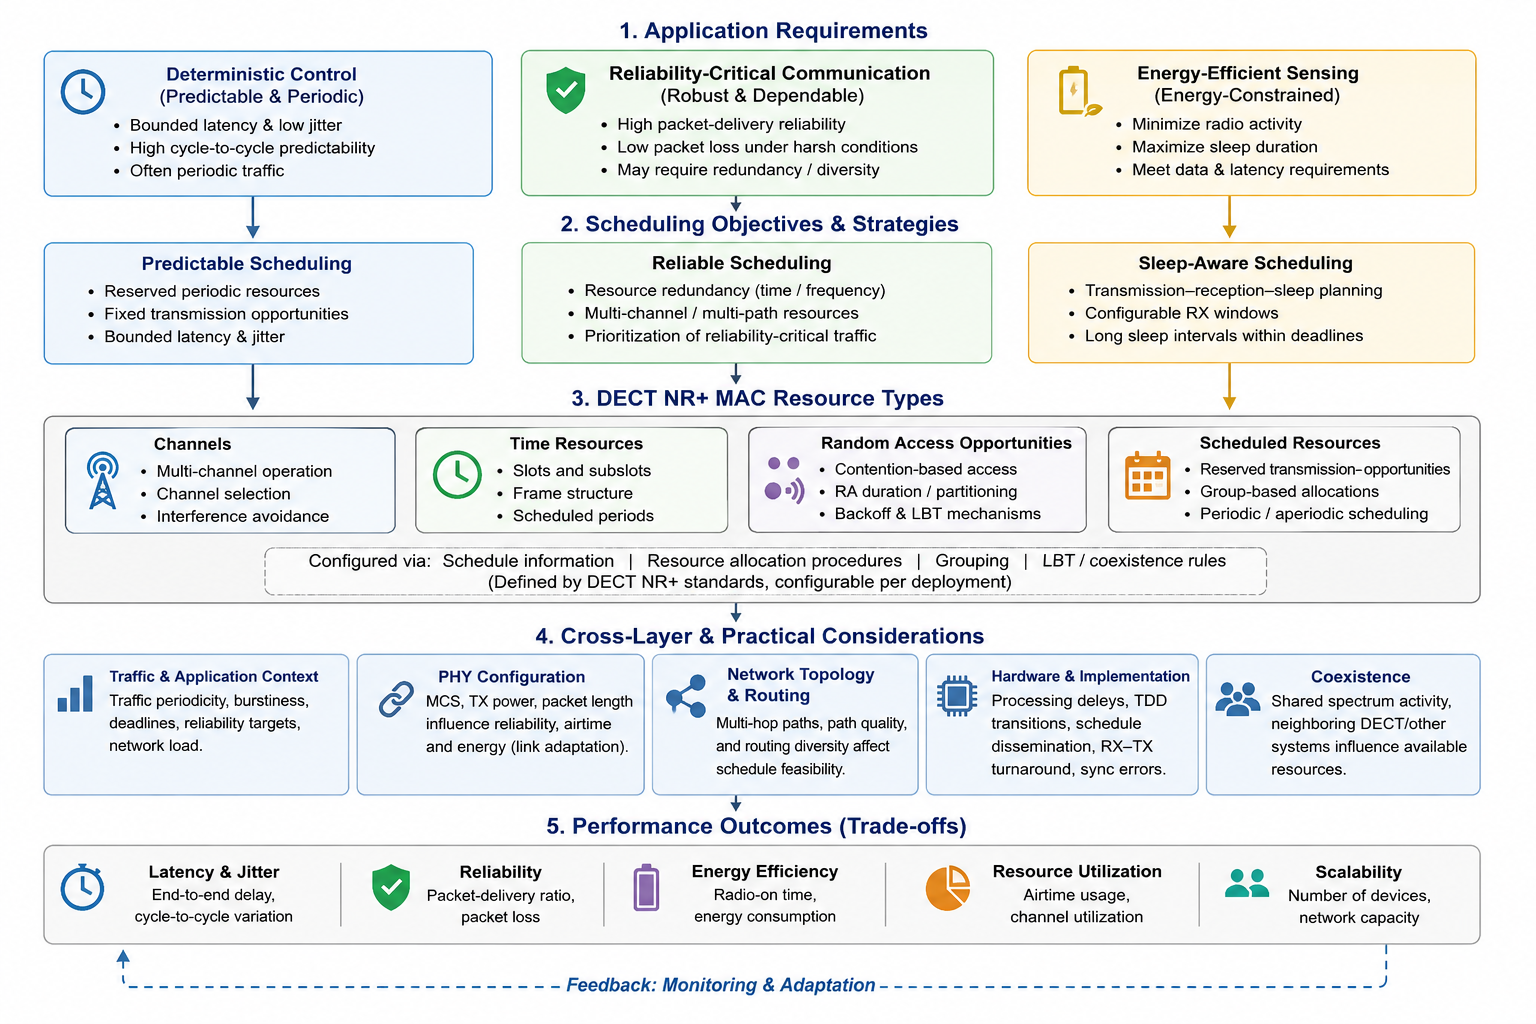
\includegraphics[width=\textwidth]{figures/app_requirments.png}
    \caption{Application-oriented scheduling and resource-allocation design
    space for DECT NR+. Application requirements motivate different scheduling
    objectives, which are realized through configurable MAC resources and are
    influenced by PHY configuration, network topology, implementation
    constraints, and coexistence conditions. The resulting configurations
    determine trade-offs among latency, reliability, energy efficiency,
    resource utilization, and scalability.}
    \label{fig:application_scheduling}
\end{figure*}

A central scheduling trade-off is the balance between contention-based and
scheduled communication. Random access accommodates bursty traffic without
permanent resource reservation but becomes less predictable as contention
increases, whereas scheduled opportunities improve temporal control at the
risk of underutilization. The appropriate balance therefore depends on traffic
periodicity, load, device population, and latency requirements
\cite{samuylovPerformanceMACLayer2024a,
gaidamakaOptimizingDelaysRandom2025}. Gaidamaka et al. illustrate dynamic
resource partitioning by using a Hidden Markov Model (HMM) to estimate device
activity and adapt the random-access-phase duration. Their numerical results
show reduced access delay while preserving more time for data transmission
\cite{gaidamakaOptimizingDelaysRandom2025}. However, the approach addresses
access-phase allocation rather than the broader problem of distributing
scheduled resources among heterogeneous applications.

Latency-sensitive resource configuration is investigated by Glazkov et al.,
who jointly evaluate LBT, backoff, power control, acknowledgement timing, and
priority queuing for near-\gls{urllc}
\cite{glazkovImprovingNearURLLCServices2025}. Their simulations report
approximately 30--80\% lower multi-hop latency and 10--20\% lower packet loss
for the combined configuration, depending on traffic conditions. This
indicates that traffic prioritization and transmission timing can materially
influence end-to-end performance, although a general scheduler mapping
heterogeneous application requirements to resource assignments is not
provided.

Resource allocation also interacts with coexistence and PHY configuration.
Samuylov et al. show that scheduled access, LBT, and last-minute channel
sensing affect spectrum sharing between DECT-2020 NR and classic DECT
\cite{samuylovPerformanceAssessmentDECT20202023}. Graf et al., meanwhile,
demonstrate experimentally that MCS, transmission power, and packet length
produce environment-dependent Pareto-optimal trade-offs among data rate,
packet delivery, and energy consumption
\cite{grafParetoOptimalityApproach2026a}. Consequently, the value of an
allocated transmission opportunity depends not only on its timing but also on
the PHY configuration and radio conditions under which it is used.

Comparable application-aware concepts are more mature in cellular resource
management. Delay-aware 5G scheduling can incorporate traffic priorities,
channel conditions, fairness, and packet delay into resource assignment
\cite{madiDelayBasedResourceAllocation2022a}, while programmable RAN
frameworks extend traffic control through classification, queueing, scheduling,
shaping, and pacing
\cite{irazabalTCRANProgrammableTraffic2024}. These approaches cannot be
transferred directly because DECT NR+ combines decentralized operation,
contention, scheduled resources, flexible FT/PT roles, and native multi-hop
communication
\cite{etsi_ts103636_1,etsi_ts103636_4}. Nevertheless, they illustrate the
broader principle that application and \gls{qos} requirements should influence
resource decisions
\cite{madiDelayBasedResourceAllocation2022a,
irazabalTCRANProgrammableTraffic2024}.

This requirement is particularly important in industrial communication,
where application periods and deadlines may not align naturally with the radio
timing structure. Predictable communication requires coordination among packet
generation, resource reservation, schedule repetition, transmission,
acknowledgement, and retransmission
\cite{etsi_ts103636_3,etsi_ts103636_4}. Reliability may additionally require
redundant opportunities or channel diversity, whereas energy-constrained
devices benefit from minimizing radio activity and maximizing sleep periods.
These objectives create competing demands on the same radio resources
\cite{glazkovImprovingNearURLLCServices2025,
samuylovEmpoweringNearURLLCIoT2025,
grafParetoOptimalityApproach2026a}.

Implementation-level timing further constrains scheduling. Alizai et al.
experimentally investigate UL/DL scheduling in DECT-2020 NR star networks
using a single-chip DECT NR+ platform, digital-storage oscilloscope
measurements, and internal modem timing analysis
\cite{alizaiMeasurementDrivenLatencyAnalysis2026}. The results isolate the
RX--TX turnaround associated with alternating reception and transmission and
show that, for short-packet and request--response traffic, this turnaround can
constitute a significant part of the latency budget. Consequently, reducing
the nominal scheduling interval does not necessarily produce a proportional
reduction in end-to-end latency on a single-transceiver device
\cite{alizaiMeasurementDrivenLatencyAnalysis2026}. These findings motivate
scheduling and architectural approaches that reduce unnecessary UL/DL
alternation, including the potential separation of UL and DL resources.

A complementary perspective is provided by analytical queueing studies.
Morozova et al. model a DECT-2020 cluster as a discrete-time queue and show
that the relative timing of packet generation and service opportunities
affects waiting time, sojourn time, and information freshness
\cite{morozovaComparisonTwoModels2026a}. Nikolaev et al. extend this
perspective using a two-phase tandem queueing model to derive the distribution,
mean, and variance of Peak Age of Information (PAoI)
\cite{nikolaevModelingDECT2020Tandem2026}. Together, these studies show that
resource allocation should consider not only instantaneous access delay and
capacity but also traffic generation, queueing, service-time variability, and
information freshness
\cite{morozovaComparisonTwoModels2026a,
nikolaevModelingDECT2020Tandem2026}.

Overall, existing studies show a progression from static resource
configuration toward context-aware management. Random-access duration can be
adapted to device activity, MAC parameters and priorities can be coordinated
for latency-sensitive traffic, coexistence affects resource availability, PHY
configuration changes the utility of allocated resources, and hardware
turnaround introduces implementation-level timing constraints
\cite{gaidamakaOptimizingDelaysRandom2025,
glazkovImprovingNearURLLCServices2025,
samuylovPerformanceAssessmentDECT20202023,
grafParetoOptimalityApproach2026a,
alizaiMeasurementDrivenLatencyAnalysis2026}. However, these contributions
address separate parts of the problem rather than providing a unified
application-oriented scheduler. A central open challenge is therefore to map
application requirements for latency, reliability, traffic periodicity, and
energy to coordinated access, resource, PHY, and timing configurations while
accounting for routing and practical hardware constraints.

%%%%%%%%%%%%%%%%%%%%%%%%%%%%%%%%%%%%%%%%%%%%%%%%%%%%%%%%%%%%%%%%%%%%%%%%%%%%%%%%

%%%%%%%%%%%%%%%%%%%%%%%%%%%%%%%%%%%%%%%%%%%%%%%%%%%%%%%%%%%%%%%%%%%%%%%%%%%%%%%%
%%%%%%%%%%%%%%%%%%%%%%%%%%%%%%%%%%%%%%%%%%%%%%%%%%%%%%%%%%%%%%%%%%%%%%%%%%%%%%%%
%%%%%%%%%%%%%%%%%%%%%%%%%%%%%%%%%%%%%%%%%%%%%%%%%%%%%%%%%%%%%%%%%%%%%%%%%%%%%%%%
\subsection{Reliability, URLLC, and mMTC}
\label{subsec:reliability}
%%%%%%%%%%%%%%%%%%%%%%%%%%%%%%%%%%%%%%%%%%%%%%%%%%%%%%%%%%%%%%%%%%%%%%%%%%%%%%%%

Reliability and latency are central objectives in \gls{dectnr} research,
particularly because the technology targets demanding \gls{imt2020} use cases
while supporting decentralized, large-scale, and multi-hop operation. As shown
in Section~\ref{sec:results}, nine of the 51 included studies explicitly
address \gls{urllc}, while five address \gls{mmtc}. The literature consistently
shows that end-to-end performance emerges from interactions among link quality,
channel access, retransmissions, resource configuration, traffic load,
routing, topology, and implementation timing
\cite{maliatsosEvaluationIMT2020Candidate2022a,
smidaETSIDECT2020Component2023,
samuylovEmpoweringNearURLLCIoT2025}.

Early studies evaluated whether DECT-2020 NR could satisfy the reliability,
latency, and connection-density requirements associated with \gls{urllc} and
\gls{mmtc} under the IMT-2020 methodology
\cite{maliatsosEvaluationIMT2020Candidate2022a,
smidaETSIDECT2020Component2023,
pennerURLLCPerformanceEvaluation2021}. These evaluations established a
feasibility baseline, while subsequent experimental studies showed that
practical reliability depends strongly on radio configuration and environment
\cite{haqueDECT2020NRLink2025,
bandaraExperimentalValidationAnalysis2025,
grafParetoOptimalityApproach2026a}. Modulation and coding, transmission power,
packet length, propagation, and interference therefore determine operating
points that trade reliability against airtime, throughput, and energy
\cite{pennerURLLCPerformanceEvaluation2021,
grafParetoOptimalityApproach2026a}.

The \gls{mmtc} literature exposes similar dependencies at larger scale. Soni
et al. evaluate multi-hop decode-and-forward communication and show that
outage probability deteriorates with increasing hop count and transmission
rate, while coding improves BER performance
\cite{soniPerformanceMultihopAssisted2021}. Singhwi et al. investigate relay
selection, association, and channel allocation in an Urban-Macro scenario and
report the most favorable SINR distribution for angle-based assignment, with
approximately 7~dB difference between the best and worst evaluated approaches
\cite{singhwiDECT2020NewRadio2021}. These results demonstrate that massive
connectivity depends not only on connection density but also on relay depth,
interference, association, and channel allocation
\cite{soniPerformanceMultihopAssisted2021,
singhwiDECT2020NewRadio2021}.

Combining high reliability with low latency becomes more difficult in
multi-hop communication because retransmissions, conservative access,
acknowledgements, and forwarding improve delivery probability or reachability
while consuming additional time and radio resources
\cite{samuylovPerformanceMACLayer2024a,
glazkovImprovingNearURLLCServices2025}. Samuylov et al. report approximately
3~ms 95th-percentile latency for direct communication under the evaluated
near-\gls{urllc} conditions, whereas multi-hop latency increases to
approximately 30~ms
\cite{samuylovEmpoweringNearURLLCIoT2025}. This illustrates the substantial
latency cost introduced by additional forwarding stages.

Biswas et al. quantify this trade-off for critical-infrastructure monitoring.
Their simulations report HARQ-based user-plane latency of approximately
10.55--25.07~ms over five hops and 15.55--38.78~ms over eight hops, depending
on packet size
\cite{biswasReliableLowLatencyCommunications2024}. Additional retransmissions
further increase latency, directly demonstrating that mechanisms intended to
recover failed packets consume part of the available latency budget. These
values remain scenario-specific because the study considers an optimized,
simulation-based mesh under controlled traffic and propagation assumptions
\cite{biswasReliableLowLatencyCommunications2024}.

Glazkov et al. investigate whether coordinated configuration of standardized
mechanisms can improve this behavior by jointly considering power control,
LBT, backoff, priority queuing, and acknowledgement timing
\cite{glazkovImprovingNearURLLCServices2025}. Their simulations report
approximately 30--80\% lower multi-hop latency and 10--20\% lower packet loss,
depending on the \gls{urllc} and \gls{mmtc} traffic conditions, with
comparatively limited impact on coexisting \gls{mmtc} traffic
\cite{glazkovImprovingNearURLLCServices2025}. The results show that
differentiated traffic treatment and coordinated MAC configuration can improve
near-\gls{urllc} performance without replacing the standardized mechanisms.

Routing provides another reliability mechanism because end-to-end performance
depends on the quality and number of links traversed. Latency-oriented path
selection and topology-aware routing therefore seek to balance reliable links
against route length
\cite{asifURLLCBasedMultiHopCommunication2025,
rauwolfTopologyAwareDeepReinforcement2026a}. Rauwolf et al. explicitly
optimize this trade-off using a topology-aware GNN+DRL framework and report
reductions of up to 19.9\% in end-to-end latency and 10\% in PER, together
with fewer transmissions relative to the evaluated baselines
\cite{rauwolfTopologyAwareDeepReinforcement2026a}. The approach remains
simulation-driven, however, leaving computational requirements, online
adaptation, and generalization to physical industrial networks open.

Reliability can also be improved by modifying connectivity. Ahmad et al.
dynamically assign intermediate FT/PT devices to reconnect nodes in outage
regions and report an outage probability below 1\% under the evaluated
conditions
\cite{ahmadMACProtocolReducing2024}. Subsequent work extends this concept
toward ultra-reliable multi-hop \gls{iiot} communication through dynamic
intermediate-device assignment and additional MAC/convergence procedures
\cite{ahmadMACLayerProtocolUltraReliable2025}. Such topology adaptation can
improve connectivity but introduces signaling, forwarding, energy, and
route-establishment overhead
\cite{ahmadMACProtocolReducing2024,
ahmadMACLayerProtocolUltraReliable2025}.

Bin Asif et al. explore a complementary approach by modifying the propagation
environment through Intelligent Reflecting Surfaces (IRS) for industrial
\gls{urllc}
\cite{binasifIRSAssistedDECT2020NR2025}. Their framework identifies shadowed
regions and assigns IRS resources together with priority-based subslot
allocation. Simulation results report improved received power and throughput
and reduced RTT relative to the considered conventional and intermediate-node
approaches
\cite{binasifIRSAssistedDECT2020NR2025}. The approach broadens the reliability
design space beyond retransmission and relaying, although IRS control,
channel estimation, mobility, synchronization, and hardware integration remain
to be experimentally demonstrated
\cite{binasifIRSAssistedDECT2020NR2025}.

For \gls{mmtc}, reliability is additionally constrained by contention as
device activity increases. Samuylov et al. demonstrate the sensitivity of MAC
performance to network density, while Gaidamaka et al. adapt the random-access
phase according to estimated device activity
\cite{samuylovPerformanceMACLayer2024a,
gaidamakaOptimizingDelaysRandom2025}. Together with the relay and link-level
studies, the evidence indicates that scalable \gls{mmtc} depends jointly on
radio robustness, relay and channel assignment, contention management, and
adaptive access
\cite{singhwiDECT2020NewRadio2021,
soniPerformanceMultihopAssisted2021,
samuylovPerformanceMACLayer2024a,
gaidamakaOptimizingDelaysRandom2025}.

The coexistence of \gls{urllc} and \gls{mmtc} traffic further requires
differentiated resource treatment. Absolute priority for latency-sensitive
traffic can disadvantage massive sensing traffic, whereas uniform treatment
can prevent \gls{urllc} flows from satisfying deadlines. Existing work shows
that traffic priority, access configuration, relay selection, and adaptive
resource management can provide differentiation
\cite{samuylovEmpoweringNearURLLCIoT2025,
glazkovImprovingNearURLLCServices2025,
singhwiDECT2020NewRadio2021}.

Taken together, the literature identifies several complementary reliability
mechanisms: robust PHY configuration, contention and acknowledgement control,
retransmission, resource prioritization, relay assignment, routing, topology
adaptation, and propagation enhancement
\cite{grafParetoOptimalityApproach2026a,
glazkovImprovingNearURLLCServices2025,
ahmadMACLayerProtocolUltraReliable2025,
rauwolfTopologyAwareDeepReinforcement2026a,
binasifIRSAssistedDECT2020NR2025}. These mechanisms operate at different
layers but affect the same end-to-end objectives and incur different costs in
latency, energy, resource utilization, and complexity
\cite{samuylovPerformanceMACLayer2024a,
grafParetoOptimalityApproach2026a,
glazkovImprovingNearURLLCServices2025}. The relevant objective is therefore
not maximum reliability in isolation, but sufficient reliability within the
latency and resource constraints of the application
\cite{soniPerformanceMultihopAssisted2021,
biswasReliableLowLatencyCommunications2024,
samuylovEmpoweringNearURLLCIoT2025}.

Overall, the literature progresses from IMT-2020 feasibility assessment and
multi-hop \gls{mmtc} toward cross-layer optimization involving access,
retransmission, traffic priority, relay assignment, routing, PHY configuration,
and propagation enhancement
\cite{maliatsosEvaluationIMT2020Candidate2022a,
singhwiDECT2020NewRadio2021,
soniPerformanceMultihopAssisted2021,
samuylovPerformanceMACLayer2024a,
samuylovEmpoweringNearURLLCIoT2025,
glazkovImprovingNearURLLCServices2025,
biswasReliableLowLatencyCommunications2024,
rauwolfTopologyAwareDeepReinforcement2026a,
binasifIRSAssistedDECT2020NR2025}. Nevertheless, much of the multi-hop
near-\gls{urllc} and massive-\gls{mmtc} evidence remains analytical or
simulation-based. Experimental studies have validated important link and
commercial-device characteristics
\cite{haqueDECT2020NRLink2025,
bandaraExperimentalValidationAnalysis2025,
grafParetoOptimalityApproach2026a,
alizaiMeasurementDrivenLatencyAnalysis2026}, but comparable large-scale
end-to-end reliability experiments remain limited.

Implementation effects become particularly important at tight latency budgets.
Measurement-driven UL/DL scheduling analysis shows that RX--TX turnaround on
single-transceiver DECT NR+ hardware can constitute a significant component of
short-packet and request--response latency
\cite{alizaiMeasurementDrivenLatencyAnalysis2026}. Such hardware delays can
accumulate with access, forwarding, queueing, acknowledgement, and
retransmission delays across multiple hops.

Future work should therefore treat reliability as an end-to-end,
application-dependent, and cross-layer property. Large-scale experiments are
needed to characterize reliability and latency under realistic interference,
heterogeneous traffic, mobility, failures, variable device activity, and
hardware timing, while jointly considering deadline-aware retransmission,
resource or path redundancy, multi-channel diversity, reliability-aware
routing, and priority-aware coexistence of \gls{urllc} and \gls{mmtc}.
%%%%%%%%%%%%%%%%%%%%%%%%%%%%%%%%%%%%%%%%%%%%%%%%%%%%%%%%%%%%%%%%%%%%%%%%%%%%%%%%
%%%%%%%%%%%%%%%%%%%%%%%%%%%%%%%%%%%%%%%%%%%%%%%%%%%%%%%%%%%%%%%%%%%%%%%%%%%%%%%%
%%%%%%%%%%%%%%%%%%%%%%%%%%%%%%%%%%%%%%%%%%%%%%%%%%%%%%%%%%%%%%%%%%%%%%%%%%%%%%%%
%%%%%%%%%%%%%%%%%%%%%%%%%%%%%%%%%%%%%%%%%%%%%%%%%%%%%%%%%%%%%%%%%%%%%%%%%%%%%%%%
\subsection{Energy Efficiency}
\label{subsec:energy}
%%%%%%%%%%%%%%%%%%%%%%%%%%%%%%%%%%%%%%%%%%%%%%%%%%%%%%%%%%%%%%%%%%%%%%%%%%%%%%%%

Energy efficiency is an important objective for \gls{dectnr}, particularly
for battery-powered sensing and \gls{mmtc} applications. As shown in
Section~\ref{sec:results}, eight of the 51 included studies address
energy-related aspects. The literature shows that communication energy depends
not only on transmission power but also on radio duty cycle, reception,
forwarding, topology, PHY configuration, retransmissions, traffic, and latency
requirements.

At the network level, Kovalchukov et al. show that multi-hop communication can
reduce transmission energy relative to direct long-range links under the
evaluated \gls{mmtc} conditions
\cite{kovalchukovDECT2020NewRadio2022}. However, increasing routing bias and
hop count also increases forwarding energy, with device density and
interference influencing the resulting balance. Multi-hop operation therefore
does not provide an unconditional energy advantage; its benefit depends on the
trade-off between shorter transmission distances and additional forwarding
activity
\cite{kovalchukovDECT2020NewRadio2022}.

Nihtila and Berg examine this trade-off from the perspective of battery-powered
mesh operation and identify a fundamental tension between communication
latency and device lifetime
\cite{nihtilaEnergyConsumptionDECT20202022}. Leaf devices carrying sporadic
traffic can remain inactive for comparatively long periods, whereas forwarding
nodes must provide sufficiently frequent receive opportunities. Shorter
availability intervals reduce forwarding latency but increase radio-on time,
creating asymmetric energy consumption between leaf and router devices
\cite{nihtilaEnergyConsumptionDECT20202022}.

To distribute this forwarding burden, Nihtila and Taipale propose periodic
router rotation among eligible nodes
\cite{nihtilaEnergySavingRouter2022}. Their simulations show that rotating
forwarding responsibility can improve the distribution of energy consumption
and extend network lifetime relative to static router assignment. This
distinguishes device-level energy efficiency from network lifetime: minimizing
aggregate communication energy does not necessarily prevent strategically
important forwarding nodes from being depleted prematurely
\cite{nihtilaEnergySavingRouter2022}. Energy-aware routing must therefore
consider both communication performance and the distribution of forwarding
cost across devices
\cite{nihtilaEnergyConsumptionDECT20202022,
nihtilaEnergySavingRouter2022}.

Experimental work complements these system-level studies with measurements on
commercial DECT NR+ hardware. Bandara reports energy costs of approximately
0.26--2.6~$\mu$J/bit depending on MCS and operating conditions, together with
measurements of range, throughput, and latency
\cite{bandaraExperimentalValidationAnalysis2025}. The approximately
order-of-magnitude variation indicates that PHY configuration strongly affects
the energy required to deliver useful information and that energy metrics
should be interpreted together with delivery reliability and application
requirements.

Graf et al. further show that modem current consumption differs substantially
across radio states and increases at high transmission power
\cite{grafWhatExpectWhen2026}. Their subsequent multi-objective analysis
jointly considers MCS, transmit power, packet length, data rate, PDR, and
energy consumption and identifies environment-dependent Pareto-optimal
configurations
\cite{grafParetoOptimalityApproach2026a}. Lower transmit power does not
necessarily minimize energy if it increases packet errors and retransmissions,
while robust configurations may increase airtime. Energy-efficient PHY
operation is therefore application- and channel-dependent rather than
represented by a universally optimal radio configuration
\cite{grafParetoOptimalityApproach2026a}.

These results connect energy directly to scheduling and reliability.
Applications with relaxed reporting deadlines can tolerate longer inactive
periods, whereas latency-sensitive communication requires more frequent radio
availability. Similarly, deteriorating channels or stringent reliability
requirements can require increased transmission power, robust modulation, or
retransmissions, each increasing energy consumption. Energy optimization must
therefore consider radio configuration, activity scheduling, and communication
requirements jointly
\cite{nihtilaEnergyConsumptionDECT20202022,
bandaraExperimentalValidationAnalysis2025,
grafParetoOptimalityApproach2026a}.

A substantially different operating regime is introduced by ambient
backscatter. Liao et al. investigate whether existing DECT NR+ transmissions
can serve as an ambient RF source for extremely low-power devices
\cite{liaoDataAssistedBackscatter2025}. Their design integrates a backscatter
receiver with a DECT NR+ SDR receiver and exploits waveform structure for
data-assisted detection. Over-the-air experiments demonstrate feasibility,
with BER values as low as 0.02 under the most favorable evaluated conditions
\cite{liaoDataAssistedBackscatter2025}. Although still a proof of concept,
this approach broadens the energy design space beyond optimization of active
radios and could support sensing devices with substantially smaller power
budgets. Practical challenges remain in range, multi-device access,
synchronization, scheduling, interference, and operation in industrial
channels
\cite{liaoDataAssistedBackscatter2025}.

The reviewed evidence can therefore be interpreted at three interacting
levels. At the device and link level, modem state, MCS, transmission power,
packet length, and delivery probability determine communication energy
\cite{bandaraExperimentalValidationAnalysis2025,
grafWhatExpectWhen2026,
grafParetoOptimalityApproach2026a}. At the network level, transmission
distance, topology, hop count, router availability, and forwarding
responsibility determine both aggregate consumption and its distribution
across devices
\cite{kovalchukovDECT2020NewRadio2022,
nihtilaEnergyConsumptionDECT20202022,
nihtilaEnergySavingRouter2022}. At the system level, ambient backscatter
extends DECT NR+-based communication toward devices with substantially lower
power budgets
\cite{liaoDataAssistedBackscatter2025}.

These findings are consistent with broader energy-efficient wireless MAC
research, where reducing idle listening, unnecessary reception, contention,
overhearing, and radio-on time is fundamental
\cite{tsaoSurveyEnergyEfficient2011}. DECT NR+ adds the complication that
native multi-hop operation makes a device's sleep schedule dependent not only
on its own traffic but also on its forwarding responsibility. Sleep-aware
scheduling, energy-aware routing, and router-role assignment are consequently
closely coupled
\cite{nihtilaEnergyConsumptionDECT20202022,
nihtilaEnergySavingRouter2022}.

Overall, the literature indicates that DECT NR+ energy efficiency is a
cross-layer property. Transmission parameters determine link-level energy;
topology and routing distribute forwarding costs; duty cycle determines
background reception energy; scheduling determines radio availability; and
reliability requirements introduce additional airtime or retransmissions
\cite{kovalchukovDECT2020NewRadio2022,
nihtilaEnergyConsumptionDECT20202022,
nihtilaEnergySavingRouter2022,
grafParetoOptimalityApproach2026a}. However, mesh-level energy and router-role
studies remain predominantly simulation-based, whereas detailed hardware
measurements mainly characterize point-to-point operation
\cite{kovalchukovDECT2020NewRadio2022,
nihtilaEnergyConsumptionDECT20202022,
nihtilaEnergySavingRouter2022,
bandaraExperimentalValidationAnalysis2025,
grafWhatExpectWhen2026,
grafParetoOptimalityApproach2026a}.

A major remaining challenge is therefore experimentally validated,
application-oriented lifetime optimization. Future work should jointly
consider sleep-aware scheduling, residual-energy-aware relay selection,
router rotation, adaptive PHY configuration, application deadlines, and
battery state. Large-scale hardware experiments are particularly needed to
determine how these mechanisms interact under realistic interference,
heterogeneous traffic, changing topology, and multi-hop operation
\cite{nihtilaEnergySavingRouter2022,
grafParetoOptimalityApproach2026a,
liaoDataAssistedBackscatter2025}.
%%%%%%%%%%%%%%%%%%%%%%%%%%%%%%%%%%%%%%%%%%%%%%%%%%%%%%%%%%%%%%%%%%%%%%%%%%%%%%%%
%%%%%%%%%%%%%%%%%%%%%%%%%%%%%%%%%%%%%%%%%%%%%%%%%%%%%%%%%%%%%%%%%%%%%%%%%%%%%%%%
%%%%%%%%%%%%%%%%%%%%%%%%%%%%%%%%%%%%%%%%%%%%%%%%%%%%%%%%%%%%%%%%%%%%%%%%%%%%%%%%
%%%%%%%%%%%%%%%%%%%%%%%%%%%%%%%%%%%%%%%%%%%%%%%%%%%%%%%%%%%%%%%%%%%%%%%%%%%%%%%%
\subsection{Positioning and Localization}
\label{subsec:positioning}
%%%%%%%%%%%%%%%%%%%%%%%%%%%%%%%%%%%%%%%%%%%%%%%%%%%%%%%%%%%%%%%%%%%%%%%%%%%%%%%%

Positioning and localization represent an emerging research direction within
\gls{dectnr}. As shown in Section~\ref{sec:results}, six of the 51 included
studies address positioning or localization, while only two are classified
primarily in this category. Compared with PHY, MAC, and routing, localization
therefore remains comparatively immature. A central challenge is to obtain
useful positioning information without excessive measurement, signaling,
processing, and energy overhead
\cite{saikkoPositioningDECT2020NR2024,
saikkoPositioningTrackingDECT20202025}.

Saikko et al. address this problem through proactive measurement selection
using time-of-arrival-based range and angle-of-arrival measurements
\cite{saikkoPositioningDECT2020NR2024}. Rather than acquiring measurements
from all available anchors, Fisher information is used together with prior
state information from an extended Kalman filter (EKF) to select measurements
expected to contribute most strongly to positioning accuracy. This differs
from SNR-based selection because a high-quality measurement may provide little
additional geometric information when it is redundant with existing
observations.

The numerical results show substantial benefits when only a limited number of
anchors is selected. With two range-measurement anchors, positioning RMSE is
approximately 47.5--62.5\% lower than with the SNR-based reference, while
three selected anchors provide approximately 20.1--31.4\% lower RMSE
\cite{saikkoPositioningDECT2020NR2024}. Tail performance also improves
substantially: with two range anchors and a 1~s measurement interval, the
99.9th-percentile positioning error is approximately 0.84~m compared with
6.13~m for SNR-based selection
\cite{saikkoPositioningDECT2020NR2024}. These results indicate that
positioning accuracy can be improved without indiscriminately increasing the
number of measurements.

Saikko et al. subsequently extend the framework toward multimodal positioning
and tracking using range, angle, and received signal strength (RSS)
measurements together with EKF- and particle-filter-based tracking
\cite{saikkoPositioningTrackingDECT20202025}. Fisher-information-based
selection again prioritizes measurements according to their expected
contribution. With two selected anchors, the reported positioning RMSE is
approximately 10--50\% lower than with SNR-based selection, depending on
measurement type and conditions, while reductions in the largest positioning
errors reach approximately 60\%
\cite{saikkoPositioningTrackingDECT20202025}. The study also shows that
selection performance depends on the quality of prior state information;
longer measurement intervals and increased prediction uncertainty can reduce
the reliability of anchor selection
\cite{saikkoPositioningTrackingDECT20202025}.

Together, these studies establish an important principle for DECT NR+
localization: positioning should optimize the \emph{information value} of
measurements rather than simply maximizing the number acquired
\cite{saikkoPositioningDECT2020NR2024,
saikkoPositioningTrackingDECT20202025}. Measurement selection consequently
becomes a resource-management problem because fewer, more informative
measurements can reduce signaling, processing, radio activity, and potentially
energy consumption while maintaining positioning performance.

Localization can also support network operation. F{\"u}hrling et al.
incorporate multi-hop localization into a routing framework for partially
known mesh topologies, using estimated relative node positions to support
local route discovery
\cite{fuhrlingRobustRoutingProtocol2025b}. This illustrates two complementary
roles for localization in DECT NR+: \emph{application-level positioning}, in
which location is the required service, and \emph{network-assisted
localization}, in which spatial information supports functions such as routing
or topology management
\cite{fuhrlingRobustRoutingProtocol2025b}.

The available evidence nevertheless remains predominantly analytical and
simulation-based
\cite{saikkoPositioningDECT2020NR2024,
saikkoPositioningTrackingDECT20202025}. Comparable large-scale localization
measurements on commercial DECT NR+ hardware in industrial environments remain
limited. This is important because NLoS propagation, metallic structures,
dynamic blockage, multipath, synchronization, antenna geometry, and mobility
can introduce measurement errors that are difficult to represent completely
through idealized models.

Positioning also interacts directly with communication resources. Increasing
measurement frequency or the number of participating anchors can improve
tracking information but consumes additional radio, processing, and energy
resources, whereas sparse measurements reduce overhead at the cost of greater
state uncertainty
\cite{saikkoPositioningDECT2020NR2024,
saikkoPositioningTrackingDECT20202025}. Localization should therefore
ultimately be treated as a joint communication--positioning resource-management
problem involving measurement modality, anchor selection, update interval,
mobility, state uncertainty, and application accuracy requirements.

Native multi-hop operation additionally creates opportunities for cooperative
localization. The use of multi-hop localization for routing already provides
an initial indication of this potential
\cite{fuhrlingRobustRoutingProtocol2025b}, but cooperative accuracy,
signaling overhead, synchronization, error propagation, and scalability remain
largely unexplored.

Overall, DECT NR+ positioning research has progressed from proactive selection
of range and angle measurements toward multimodal range--angle--RSS tracking.
Information-aware measurement selection can substantially improve positioning
performance when measurement resources are limited
\cite{saikkoPositioningDECT2020NR2024,
saikkoPositioningTrackingDECT20202025}, but experimental maturity remains
considerably below that of communication-oriented DECT NR+ research. Future
work should therefore emphasize hardware-based industrial localization,
mobility and NLoS conditions, multimodal fusion, adaptive measurement
intervals, cooperative mesh positioning, and integration of positioning with
MAC scheduling and energy management.
%%%%%%%%%%%%%%%%%%%%%%%%%%%%%%%%%%%%%%%%%%%%%%%%%%%%%%%%%%%%%%%%%%%%%%%%%%%%%%%%
%%%%%%%%%%%%%%%%%%%%%%%%%%%%%%%%%%%%%%%%%%%%%%%%%%%%%%%%%%%%%%%%%%%%%%%%%%%%%%%%
%%%%%%%%%%%%%%%%%%%%%%%%%%%%%%%%%%%%%%%%%%%%%%%%%%%%%%%%%%%%%%%%%%%%%%%%%%%%%%%%
%%%%%%%%%%%%%%%%%%%%%%%%%%%%%%%%%%%%%%%%%%%%%%%%%%%%%%%%%%%%%%%%%%%%%%%%%%%%%%%%
\subsection{Security, Coexistence, and Multi-RAT Integration}
\label{subsec:security_coexistence}
%%%%%%%%%%%%%%%%%%%%%%%%%%%%%%%%%%%%%%%%%%%%%%%%%%%%%%%%%%%%%%%%%%%%%%%%%%%%%%%%

Security, coexistence, and heterogeneous-network integration remain
comparatively underexplored in the \gls{dectnr} literature. As shown in
Section~\ref{sec:results}, only three of the 51 included studies were coded
under security or multi-RAT integration, while two explicitly address
coexistence or regulatory aspects. Compared with PHY, MAC, and routing, these
deployment-oriented topics therefore remain relatively immature.

Security functionality is nevertheless integral to the standardized DECT NR+
architecture. The specifications define mechanisms for device identification,
authentication, key management, integrity protection, and confidentiality
\cite{etsi_ts103636_4,etsi_ts103636_5}. In multi-hop networks, however,
security extends beyond individual radio links because devices can participate
in forwarding, topology formation, relay selection, and dynamic FT/PT
relationships. Increasingly sophisticated routing mechanisms based on topology
and link information consequently depend on the trustworthiness of distributed
network state
\cite{fuhrlingRobustRoutingProtocol2025b,
rauwolfTopologyAwareDeepReinforcement2026a}.

Comparable threats are well established in other low-power mesh networks,
where manipulation of routing information has motivated lightweight detection
mechanisms for attacks such as rank manipulation
\cite{kalyaniResourceefficientEnsembleMachine2026}. Although such mechanisms
cannot be transferred directly to DECT NR+, they illustrate the need to
evaluate routing manipulation, falsified topology information, unauthorized
participation, and resource-exhaustion attacks in distributed DECT NR+
networks.

Ngo addresses security from an interworking perspective by integrating
resource-constrained non-cellular IoT devices, including DECT-2020 NR
platforms, with 5G-core authentication and session management
\cite{ngoIoTDeviceAuthentication2025}. The architecture transfers substantial
authentication and traffic-control functionality toward the 5G core rather
than requiring a complete cellular security stack on every constrained device,
and interoperability is demonstrated with commercial and open-source 5G core
platforms
\cite{ngoIoTDeviceAuthentication2025}. Although this work is used here as
contextual evidence rather than as part of the 51-study primary corpus, it
provides a relevant pathway for incorporating DECT NR+-based devices into
broader infrastructure-managed security architectures.

A second deployment challenge is spectrum coexistence. DECT NR+ channel
access depends on sensing, LBT, backoff, and resource-selection procedures,
which influence both internal performance and interaction with other spectrum
users
\cite{etsi_ts103636_2,etsi_ts103636_4}. Samuylov et al. evaluate coexistence
between DECT-2020 NR and classic DECT using LBT, last-minute scanning, and
scheduling-based mechanisms
\cite{samuylovPerformanceAssessmentDECT20202023}. Under the evaluated
conditions, standard LBT keeps classic-DECT packet drops below approximately
2\% when 25\% of resources are allocated to classic DECT. Last-minute
scanning increases DECT-2020 NR packet drops by more than 10\% relative to
LBT-only operation, whereas the considered scheduling approach improves
DECT-2020 NR performance by approximately 2--5\%
\cite{samuylovPerformanceAssessmentDECT20202023}. These results indicate
that coexistence performance depends on the particular sensing and scheduling
strategy rather than channel occupancy alone
\cite{samuylovPerformanceAssessmentDECT20202023,
samuylovPerformanceMACLayer2024a}.

Regulatory access rules can impose additional constraints. Samuylov et al.
compare native DECT-2020 NR LBT with mesh operation following FCC access rules
for the UPCS band
\cite{samuylovPerformanceDECT2020NR2025}. In the evaluated scenarios,
packet delivery for the FCC-based mesh falls below 85\%, compared with
approximately 98--99\% using native DECT NR+ LBT, while the effect on
coexisting classic-DECT devices remains comparatively small
\cite{samuylovPerformanceDECT2020NR2025}. The result shows that practical
mesh performance depends not only on the radio protocol but also on the
regulatory spectrum-access regime.

A third direction concerns deliberate cooperation between DECT NR+ and other
\glspl{rit}. Rather than using one technology for every function,
heterogeneous architectures can exploit complementary capabilities: DECT NR+
for decentralized discovery and direct or multi-hop communication, Wi-Fi for
high-throughput local transfer, and 5G infrastructure for authentication,
session management, and external connectivity.

Dang et al. demonstrate this principle through enhanced wireless direct
connectivity (EWDC), which combines DECT-2020 NR and Wi-Fi
\cite{dangEWDCIntegratingDECT20202025a}. DECT is used for discovery and secure
exchange of Wi-Fi configuration information, while Wi-Fi carries the
high-bandwidth data path. The implementation uses Nordic nRF9161-DK hardware,
with WireGuard protecting Wi-Fi communication
\cite{dangEWDCIntegratingDECT20202025a}. EWDC therefore illustrates a
functional division between control/discovery and data transmission rather
than requiring both radios to carry identical traffic.

The subsequent Uni-RAT framework extends this concept to DECT-2020 NR,
Wi-Fi, and a 5G core
\cite{dangUniRATUnifiedDECT20202026}. DECT-2020 NR operates as the Master-RAT
and anchors control-plane security through 5G-AKA and NAS, while Wi-Fi acts as
a Secondary-RAT for data delivery. WireGuard protects Layer-3 communication,
and customized NAS signaling distributes configuration and keying information.
A physical prototype combines Nordic nRF9161 DECT devices, Raspberry Pi Wi-Fi
nodes, a commercial 5G core, and Arm TrustZone for security-critical
functionality
\cite{dangUniRATUnifiedDECT20202026}.

Taken together, the interworking studies indicate a progression from
core-assisted authentication toward functional and security integration across
DECT NR+, Wi-Fi, and 5G infrastructure
\cite{ngoIoTDeviceAuthentication2025,
dangEWDCIntegratingDECT20202025a,
dangUniRATUnifiedDECT20202026}. Such integration also expands the trust
boundary across radio interfaces, gateways, security contexts, configuration
exchange, and core-network functions. Multi-RAT systems must additionally
decide which interface should carry a traffic flow and when another RAT should
be activated according to application requirements and radio conditions
\cite{dangEWDCIntegratingDECT20202025a,
dangUniRATUnifiedDECT20202026}.

The available evidence can therefore be synthesized across three interacting
deployment dimensions. \emph{Security} determines trusted participation and
communication protection
\cite{etsi_ts103636_4,etsi_ts103636_5,
ngoIoTDeviceAuthentication2025}; \emph{coexistence} determines how DECT NR+
shares spectrum under technical and regulatory constraints
\cite{samuylovPerformanceAssessmentDECT20202023,
samuylovPerformanceDECT2020NR2025}; and \emph{multi-RAT integration}
determines how DECT NR+ cooperates with complementary radio and core-network
technologies
\cite{dangEWDCIntegratingDECT20202025a,
dangUniRATUnifiedDECT20202026}. These dimensions are coupled because
interference can trigger channel or RAT changes, inter-RAT transitions can
require security procedures, and authentication and tunneling introduce
processing and signaling overhead.

Despite recent progress, experimental evidence remains limited. Coexistence
studies are predominantly simulation-based
\cite{samuylovPerformanceAssessmentDECT20202023,
samuylovPerformanceDECT2020NR2025}, whereas security and multi-RAT prototypes
cover only a subset of possible authentication, mobility, failover, routing,
and heterogeneous-traffic scenarios
\cite{ngoIoTDeviceAuthentication2025,
dangEWDCIntegratingDECT20202025a,
dangUniRATUnifiedDECT20202026}. Security of native multi-hop operation is a
particularly important gap because increasingly sophisticated routing and
topology-management mechanisms have not yet been matched by comparable
attack-oriented experimental analysis
\cite{fuhrlingRobustRoutingProtocol2025b,
rauwolfTopologyAwareDeepReinforcement2026a}.

Overall, the evidence shows a progression from standardized security and
autonomous spectrum access toward heterogeneous connectivity architectures.
Coexistence and regulatory constraints can materially affect packet-delivery
performance, while core-assisted authentication, EWDC, and Uni-RAT demonstrate
practical pathways for integrating DECT NR+ with Wi-Fi and 5G infrastructure
\cite{samuylovPerformanceAssessmentDECT20202023,
samuylovPerformanceDECT2020NR2025,
ngoIoTDeviceAuthentication2025,
dangEWDCIntegratingDECT20202025a,
dangUniRATUnifiedDECT20202026}. Future research should emphasize secure
multi-hop operation, attack-oriented evaluation, interference-aware channel
selection, application-aware RAT selection, mobility and failover, and
experimental characterization of the latency, energy, and signaling overhead
introduced by security and interworking mechanisms.
%%%%%%%%%%%%%%%%%%%%%%%%%%%%%%%%%%%%%%%%%%%%%%%%%%%%%%%%%%%%%%%%%%%%%%%%%%%%%%%%
%%%%%%%%%%%%%%%%%%%%%%%%%%%%%%%%%%%%%%%%%%%%%%%%%%%%%%%%%%%%%%%%%%%%%%%%%%%%%%%%
%%%%%%%%%%%%%%%%%%%%%%%%%%%%%%%%%%%%%%%%%%%%%%%%%%%%%%%%%%%%%%%%%%%%%%%%%%%%%%%%
%%%%%%%%%%%%%%%%%%%%%%%%%%%%%%%%%%%%%%%%%%%%%%%%%%%%%%%%%%%%%%%%%%%%%%%%%%%%%%%%
\subsection{Industrial Applications and Experimental Implementations}
\label{subsec:industrial_experimental}
%%%%%%%%%%%%%%%%%%%%%%%%%%%%%%%%%%%%%%%%%%%%%%%%%%%%%%%%%%%%%%%%%%%%%%%%%%%%%%%%

Experimental and application-oriented research provides an important measure
of the technological maturity of \gls{dectnr}. As shown in
Section~\ref{sec:results}, 14 of the 51 included studies have an industrial or
application-oriented primary contribution, while 18 address experimental,
testbed, or application aspects. Across the corpus, 16 studies employ hardware
prototypes, 11 use commercial devices, five report field-trial activities, and
three include measurements in industrial environments. The literature has
therefore progressed beyond standardization and simulation, although the scale
and realism of experimental validation vary considerably.

Industrial propagation measurements provide one important source of empirical
evidence. Wa{\ss}mann et al. investigate DECT-2020 NR at 450, 1350, and
3700~MHz using MATLAB/GNU Radio and USRP B210 hardware and report an average
RMS delay spread of approximately 65~ns for the 13.824~MHz configuration
\cite{wassmannPerformanceDECT2020NR2024}. Haque et al. complement these
measurements with practical range evaluation, demonstrating packet-success
rates above 90\% for indoor NLoS communication beyond 60~m at 0~dBm and
outdoor LoS communication beyond 600~m at 19~dBm
\cite{haqueDECT2020NRLink2025}. Together, these studies demonstrate substantial
coverage potential while confirming the strong dependence of practical
performance on propagation conditions and radio configuration.

Commercial-device experiments broaden this evidence to multiple \glspl{kpi}.
Bandara evaluates Nordic nRF91-series hardware and reports outdoor LoS
communication of approximately 730~m at an 80\% packet-delivery ratio, maximum
measured throughput of approximately 2.50~Mbit/s for MCS~4 with eight subslots
compared with approximately 3.36~Mbit/s theoretically, and a minimum measured
RTT of approximately 2.255~ms for a 12-byte payload
\cite{bandaraExperimentalValidationAnalysis2025}. Energy consumption varies
from approximately 0.26 to 2.6~$\mu$J/bit depending on configuration,
illustrating that range, throughput, latency, reliability, and energy must be
interpreted jointly.

Graf et al. similarly characterize practical radio behavior and power
consumption on commercial DECT NR+ hardware
\cite{grafWhatExpectWhen2026}. Their subsequent measurement-driven
multi-objective analysis evaluates MCS, transmit power, and packet length and
identifies environment-dependent Pareto-optimal configurations across data
rate, packet delivery, and energy consumption
\cite{grafParetoOptimalityApproach2026a}. These studies represent a transition
from hardware characterization toward experimentally informed configuration
according to application requirements.

Application-oriented prototypes provide a further level of validation.
Mudriievskyi et al. construct a low-cost DECT NR+ testbed for Tactile Internet
and human-in-the-loop communication using commercial platforms
\cite{mudriievskyiCHEAP5GDECT2024a}. Their non-optimized COTS implementation
achieves approximately 2--8~ms latency and 2.3--2.5~Mbit/s under the evaluated
packet lengths and MCS configurations
\cite{mudriievskyiCHEAP5GDECT2024a}. Although limited to two platforms and
primarily point-to-point communication, the experiment demonstrates practical
low-latency operation on comparatively inexpensive hardware.

Professional live audio constitutes another application domain with stringent
latency and reliability requirements. D{\"u}rre and Werner explore the
DECT-2020 NR design space for professional live audio using Nordic nRF91-series
modem hardware and practical latency measurements
\cite{durreDECT2020NRProfessional2024}. Their evaluation considers the
trade-off among latency, RF-resource utilization, and transmission robustness
and identifies a minimum measured latency of approximately 2.312~ms with the
available modem implementation, at the cost of roughly one third of the RF
channel resources
\cite{durreDECT2020NRProfessional2024}. Because the implementation available
for the study primarily exposed PHY-level functionality, the reported value
should be interpreted as a minimum implementation-latency estimate rather than
a complete application-level audio delay.

Poets and Wa{\ss}mann subsequently broaden the professional-audio perspective
by examining the DECT NR+ design space for wireless microphones and media
applications
\cite{poetsDECTNRNew2024}. Later work implements a functional prototype
connecting two Dante-enabled audio devices through an open-source DECT NR+ SDR
implementation
\cite{poetsProfessionalNetworkedAudio2025}. The prototype achieves an average
one-way latency of approximately 1.7~ms
\cite{poetsProfessionalNetworkedAudio2025}. Unlike isolated PHY or packet
measurements, this application-level demonstration additionally exposes
synchronization, periodic traffic, buffering, and application-specific
\gls{qos} requirements. Taken together, the professional-audio studies show a
progression from radio-level design-space exploration and modem latency
measurement toward end-to-end application prototyping
\cite{durreDECT2020NRProfessional2024,
poetsDECTNRNew2024,
poetsProfessionalNetworkedAudio2025}.

Power-grid monitoring extends experimental validation toward multi-hop and
heterogeneous application traffic. Pires et al. evaluate DECT-2020 NR mesh
networking for temperature and humidity monitoring, video-based intrusion
detection, and power-quality monitoring
\cite{piresDECT2020NREnergy2026b}. Under two-hop conditions, the three
substation use cases exhibit mean mesh latencies of approximately 15.45,
18.55, and 27.93~ms and corresponding end-to-end mean latencies of
approximately 26.6, 29.71, and 39.62~ms
\cite{piresDECT2020NREnergy2026b}. The difference illustrates the additional
delay introduced by gateway and backhaul components beyond the DECT NR+ mesh
itself. A second proof of concept uses five nRF9151/nRF9161-based nodes in a
four-hop mesh and includes a 48-hour power-quality measurement experiment,
providing evidence beyond short-duration point-to-point testing
\cite{piresDECT2020NREnergy2026b}.

The application landscape also extends beyond fixed industrial and indoor
deployments. Jahangir investigates DECT NR+ connectivity for unmanned aerial
vehicles through analytical link-budget modeling and simulation of
air-to-ground and air-to-air communication
\cite{jahangirAnalysisPerformanceDECT2024}. The analysis considers frequencies
of 915~MHz, 1.89~GHz, and 3.5~GHz together with different modulation schemes and
communication distances. Under the modeled conditions, lower-frequency
operation, particularly at 915~MHz, provides more favorable long-range link
behavior because of reduced path loss, whereas the higher-frequency options
become increasingly constrained as distance grows
\cite{jahangirAnalysisPerformanceDECT2024}. The study broadens the potential
application space of DECT NR+ toward aerial connectivity, but its evidence
remains analytical and simulation-based; UAV flight tests, mobility,
altitude-dependent propagation, antenna orientation, Doppler effects, and
dynamic routing remain open for experimental validation
\cite{jahangirAnalysisPerformanceDECT2024}.

Implementation-oriented research also addresses the realization of individual
PHY functions. Fagerholm et al. propose an FPGA-oriented synchronization
architecture requiring only two complex multiplications
\cite{fagerholmFPGAbasedDECT2020New2024}. Evaluation with MATLAB, Icarus
Verilog, and captured real-world data indicates an additional SNR requirement
of approximately 2.6~dB or more depending on configuration
\cite{fagerholmFPGAbasedDECT2020New2024}. The work demonstrates efficient
hardware-oriented synchronization, although it should not be interpreted as a
complete FPGA-based DECT NR+ PHY/MAC testbed.

Recent measurement-driven work extends experimentation toward internal
scheduling behavior. Alizai et al. investigate UL/DL scheduling on a
single-chip DECT NR+ platform using digital-storage-oscilloscope measurements
and internal modem timing analysis
\cite{alizaiMeasurementDrivenLatencyAnalysis2026}. By isolating the RX--TX
turnaround associated with alternating reception and transmission, the study
shows that hardware switching can constitute a significant component of the
latency budget for short-packet and request--response communication
\cite{alizaiMeasurementDrivenLatencyAnalysis2026}. Consequently, reducing
nominal scheduling delay alone does not necessarily produce a proportional
reduction in application-visible latency on single-transceiver hardware,
motivating scheduling and architectural approaches that reduce unnecessary
UL/DL alternation.

The experimental literature therefore spans complementary implementation
platforms. Commercial Nordic nRF91-series devices provide standardized modem
realism
\cite{durreDECT2020NRProfessional2024,
bandaraExperimentalValidationAnalysis2025,
grafWhatExpectWhen2026,
mudriievskyiCHEAP5GDECT2024a,
piresDECT2020NREnergy2026b}; SDR platforms provide greater PHY and
application-level flexibility
\cite{wassmannPerformanceDECT2020NR2024,
poetsProfessionalNetworkedAudio2025}; and FPGA-oriented work provides
architectural control over digital implementation
\cite{fagerholmFPGAbasedDECT2020New2024}. These approaches collectively show
a maturation from radio characterization toward measurement-driven
configuration and application-level validation. The UAV analysis complements
these hardware studies by illustrating how analytical modeling can be used to
explore application domains that have not yet reached physical deployment
\cite{jahangirAnalysisPerformanceDECT2024}.

Across application domains, different studies expose different aspects of
DECT NR+. Tactile communication emphasizes short-packet latency; professional
audio adds stringent periodic traffic, synchronization, and RF-resource
constraints; power-grid monitoring introduces heterogeneous traffic, gateways,
multi-hop communication, and longer-duration operation; UAV analysis introduces
mobility-oriented range and frequency considerations; industrial measurements
expose realistic propagation; and device-level studies reveal implementation
and energy constraints
\cite{wassmannPerformanceDECT2020NR2024,
haqueDECT2020NRLink2025,
bandaraExperimentalValidationAnalysis2025,
mudriievskyiCHEAP5GDECT2024a,
durreDECT2020NRProfessional2024,
poetsProfessionalNetworkedAudio2025,
piresDECT2020NREnergy2026b,
jahangirAnalysisPerformanceDECT2024,
grafWhatExpectWhen2026,
alizaiMeasurementDrivenLatencyAnalysis2026}. Application suitability should
therefore be established through use-case-specific requirements rather than a
generic claim of industrial applicability.

Despite this progress, experimental maturity remains uneven. Many hardware
studies involve small device populations, static topologies, limited traffic
diversity, or controlled radio conditions. Moreover, differences in MCS,
transmit power, payload, topology, hop count, offered load, interference, and
measurement duration make direct comparison difficult. Some application
domains, such as UAV connectivity, remain primarily model-based rather than
experimentally demonstrated
\cite{jahangirAnalysisPerformanceDECT2024}. Reproducible benchmark scenarios
and clearly defined measurement boundaries are therefore needed, particularly
because gateway, backhaul, transport, and application processing can contribute
substantially to end-to-end latency
\cite{piresDECT2020NREnergy2026b}.

Overall, DECT NR+ research has progressed from conceptual and simulation-based
feasibility toward industrial-channel measurements, commercial-device
characterization, SDR implementations, application prototypes, multi-hop
proofs of concept, and implementation-level timing analysis
\cite{durreDECT2020NRProfessional2024,
jahangirAnalysisPerformanceDECT2024}. The central experimental question is
consequently shifting from whether DECT NR+ can operate to how its PHY, MAC,
scheduling, routing, topology, and hardware configuration should be selected
for specific applications.

Future work should emphasize larger and more representative physical
deployments with multi-hop communication, mobility, heterogeneous traffic,
interference, failures, multi-channel operation, and long-duration
measurements. Experimental evaluation should jointly characterize latency
distributions, jitter, reliability, throughput, energy, and network lifetime
and explicitly map these \glspl{kpi} to application requirements. Such
reproducible, application-driven validation is necessary to determine which
combinations of DECT NR+ mechanisms provide predictable performance in real
industrial systems.
\section{Comparative Analysis}
\label{sec:comparison}

%%%%%%%%%%%%%%%%%%%%%%%%%%%%%%%%%%%%%%%%%%%%%%%%%%%%%%%%%%%%%%%

\input{sections/06_research_gaps}
\section{Future Research Directions}
\label{sec:future}

%%%%%%%%%%%%%%%%%%%%%%%%%%%%%%%%%%%%%%%%%%%%%%%%%%%%%%%%%%%%%%%

\input{sections/08_conclusion}
\printnoidxglossary[
    type=\acronymtype,
    title={List of Acronyms}
]
\bibliographystyle{elsarticle-num}
\bibliography{references}

\end{document}
